\documentclass[10pt,A4]{article}
\usepackage[top=0.85in,left=2.75in,footskip=0.75in]{geometry}

% Use adjustwidth environment to exceed column width (see example table in text)
\usepackage{changepage}

% Use Unicode characters when possible
\usepackage[utf8]{inputenc}
\usepackage{booktabs,caption,fixltx2e}
\usepackage[flushleft]{threeparttable}
\usepackage{tabularx}
% textcomp package and marvosym package for additional characters
\usepackage{textcomp,marvosym}

% fixltx2e package for \textsubscript
\usepackage{fixltx2e}

% amsmath and amssymb packages, useful for mathematical formulas and symbols
\usepackage{amsmath,amssymb}

% cite package, to clean up citations in the main text. Do not remove.
\usepackage{cite}

% Use nameref to cite supporting information files (see Supporting Information section for more info)
\usepackage{nameref,hyperref}

% line numbers
\usepackage[right]{lineno}

% ligatures disabled
\usepackage{microtype}
%\DisableLigatures[f]{encoding = *, family = * }

% rotating package for sideways tables
\usepackage{rotating}

% Remove comment for double spacing
\usepackage{setspace} 
\doublespacing

% Text layout
\raggedright
\setlength{\parindent}{0.5cm}
\textwidth 5.25in 
\textheight 8.75in

% Bold the 'Figure #' in the caption and separate it from the title/caption with a period
% Captions will be left justified
\usepackage[aboveskip=1pt,labelfont=bf,labelsep=period,justification=raggedright,singlelinecheck=off]{caption}

% Use the PLoS provided BiBTeX style
\bibliographystyle{plos2015}

% Remove brackets from numbering in List of References
\makeatletter
\renewcommand{\@biblabel}[1]{\quad#1.}
\makeatother

% Leave date blank
\date{}

% Header and Footer with logo
\usepackage{lastpage,fancyhdr,graphicx}
\usepackage{ragged2e}

\usepackage{color}
\usepackage[dvipsnames]{xcolor}

%\usepackage{epstopdf}
\pagestyle{myheadings}
\pagestyle{fancy}
\fancyhf{}
\lhead{
%
\includegraphics[width=1.6in]{figures/pone.png}
}
\rhead{Calibration of a Density-based Model of Urban Morphogenesis\vspace{2mm}}
\rfoot{\thepage}
\renewcommand{\footrule}{\hrule height 2pt \vspace{2mm}}
\fancyheadoffset[L]{2.25in}
\fancyfootoffset[L]{2.25in}
%\lfoot{\sf Raimbault, 2017}
\lfoot{}

%% Include all macros below

\newcommand{\lorem}{{\bf LOREM}}
\newcommand{\ipsum}{{\bf IPSUM}}

%%%%%%%%%%%%%%%%%%%%%%
%% User-defined commands
%%%%%%%%%%%%%%%%%%%%%%


%Yoann's commands
\newcommand{\reels}{\mathbb{R}}
\newcommand{\naturels}{\mathbb{N}}
\newcommand{\relatifs}{\mathbb{Z}}
\newcommand{\rat}{\mathbb{Q}}
\newcommand{\complex}{\mathbb{C}}
\newcommand{\esp}{\mathbb{E}}
\newcommand{\proba}{\mathbb{P}}
\newcommand{\var}{\operatorname{Var}}
\newcommand{\cov}{\operatorname{Cov}}
\newcommand{\Tau}{\mathrm{T}}



% writing utilities

% comments and responses
\usepackage{xparse}
\DeclareDocumentCommand{\comment}{m o o o o}
{%
    \textcolor{red}{#1}
    \IfValueT{#2}{\textcolor{blue}{#2}}
    \IfValueT{#3}{\textcolor{ForestGreen}{#3}}
    \IfValueT{#4}{\textcolor{red!50!blue}{#4}}
    \IfValueT{#5}{\textcolor{Aquamarine}{#5}}
}


% todo
\newcommand{\todo}[1]{\textcolor{red!50!blue}{\textbf{\textit{#1}}}}




%% END MACROS SECTION


\begin{document}
\vspace*{0.35in}


\justify









%\end{document}





\section*{S1 Text : Extended Figures for Model Exploration}


\subsection*{Convergence}

% histograms


% and bimodal statistical distribution for cumulated points in the parameter space confirm the existence of superposed regimes : gaussian distribution gives stationary configurations, whereas inverse log-normal distribution are close to real data shape and correspond to non-stationary regime.
% -> not sure it is interesting to look at cumulated histograms.

% Figures :

%%%%%%%%%%%%%%%%%%%%
\begin{figure}
\centering
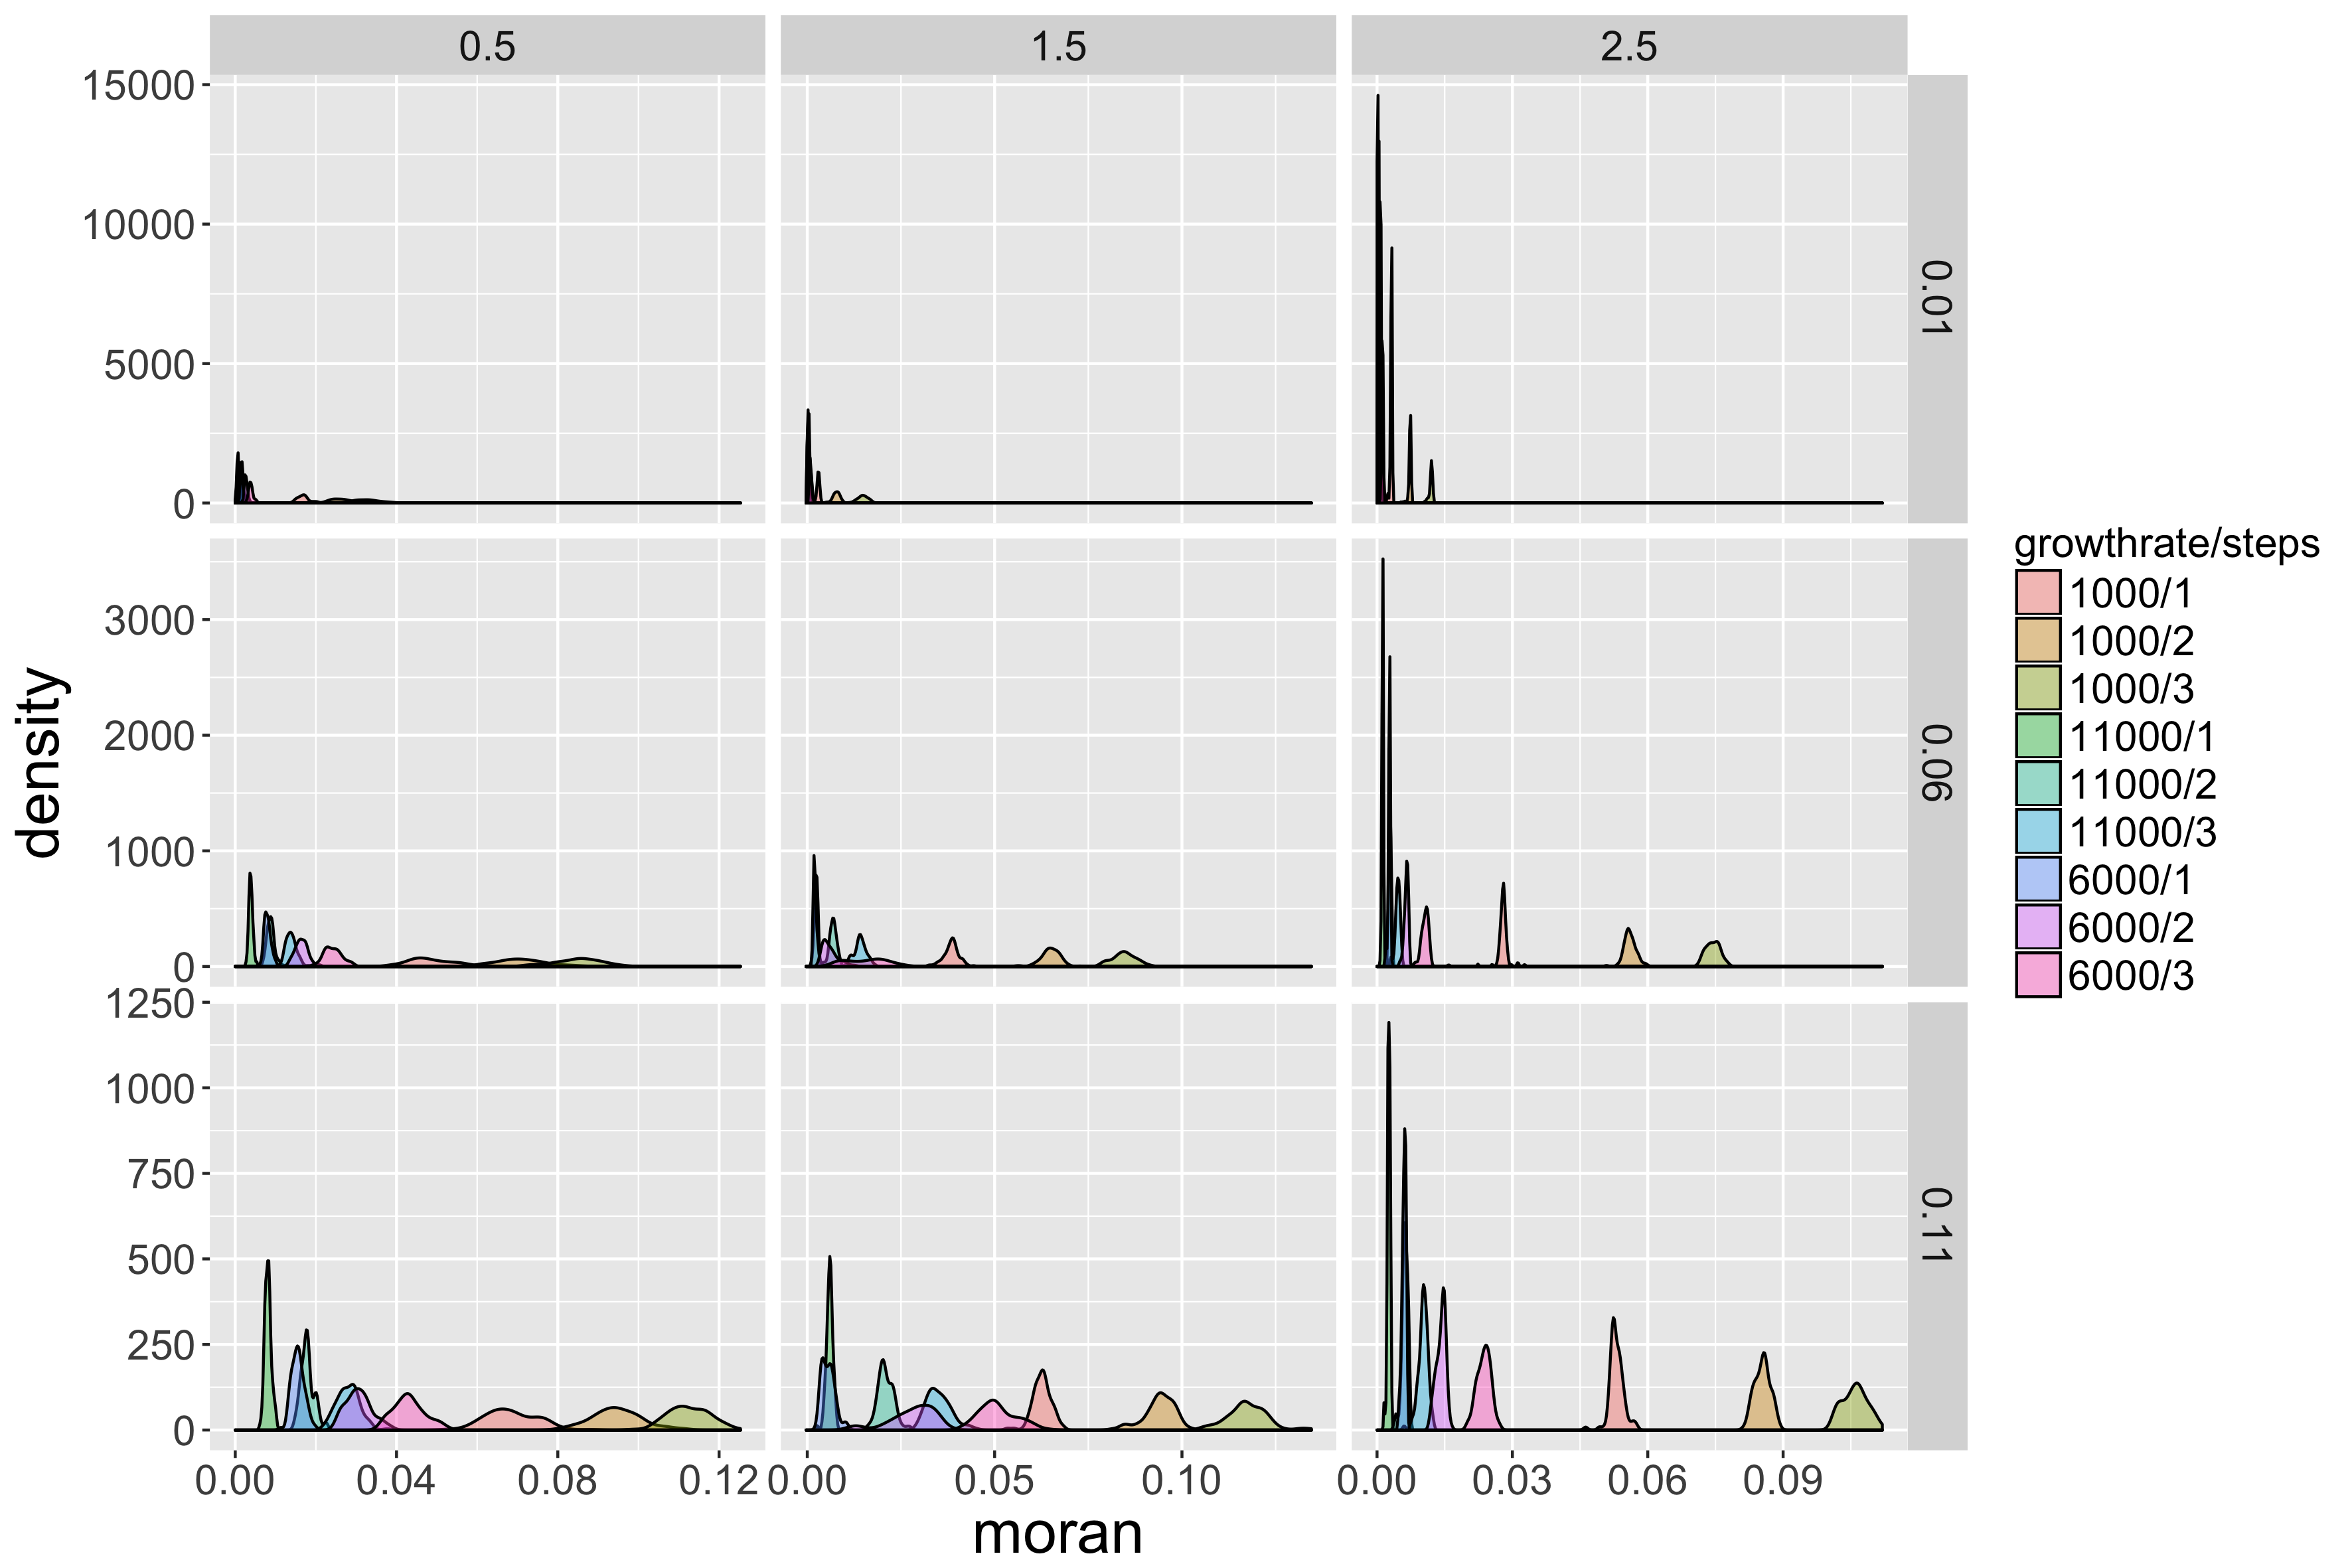
\includegraphics[width=\textwidth]{figuresraw/hist_moran}\\
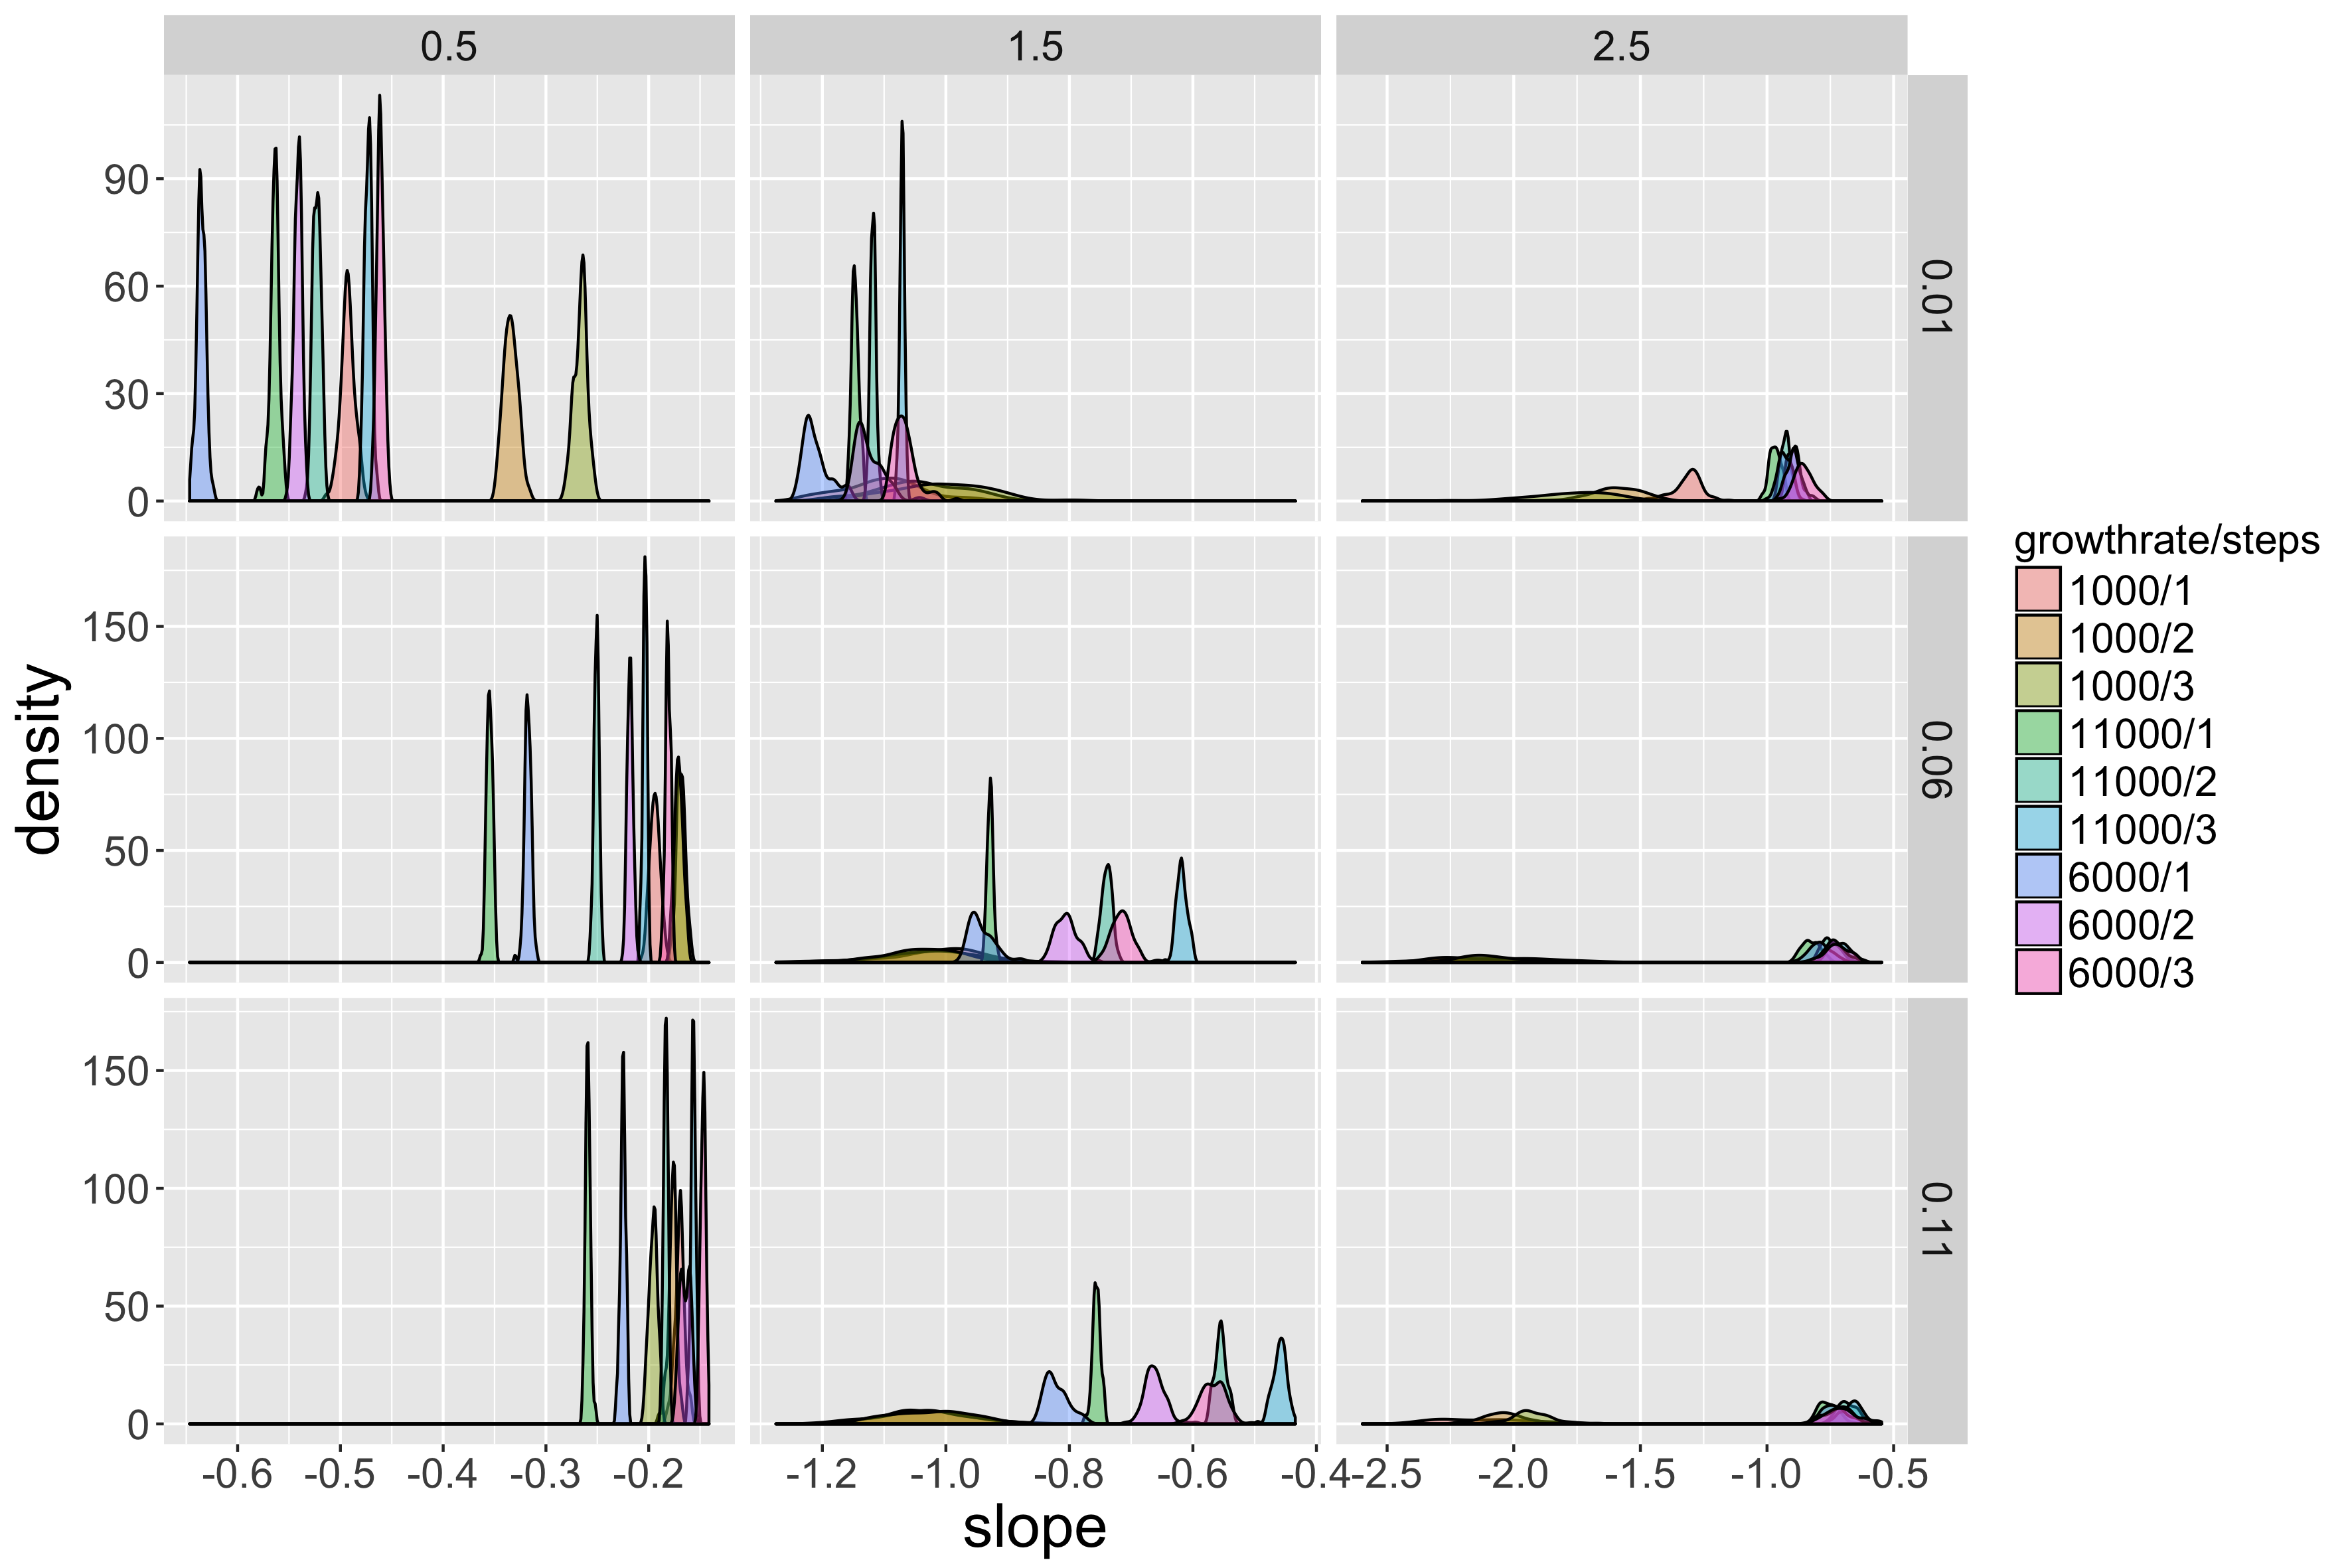
\includegraphics[width=\textwidth]{figuresraw/hist_slope}
\caption{}
\label{}
\end{figure}
%%%%%%%%%%%%%%%%%%%%






\subsection*{Indicators Scatterplots}

% scatterplots - with real points


%%%%%%%%%%%%%
\begin{figure}
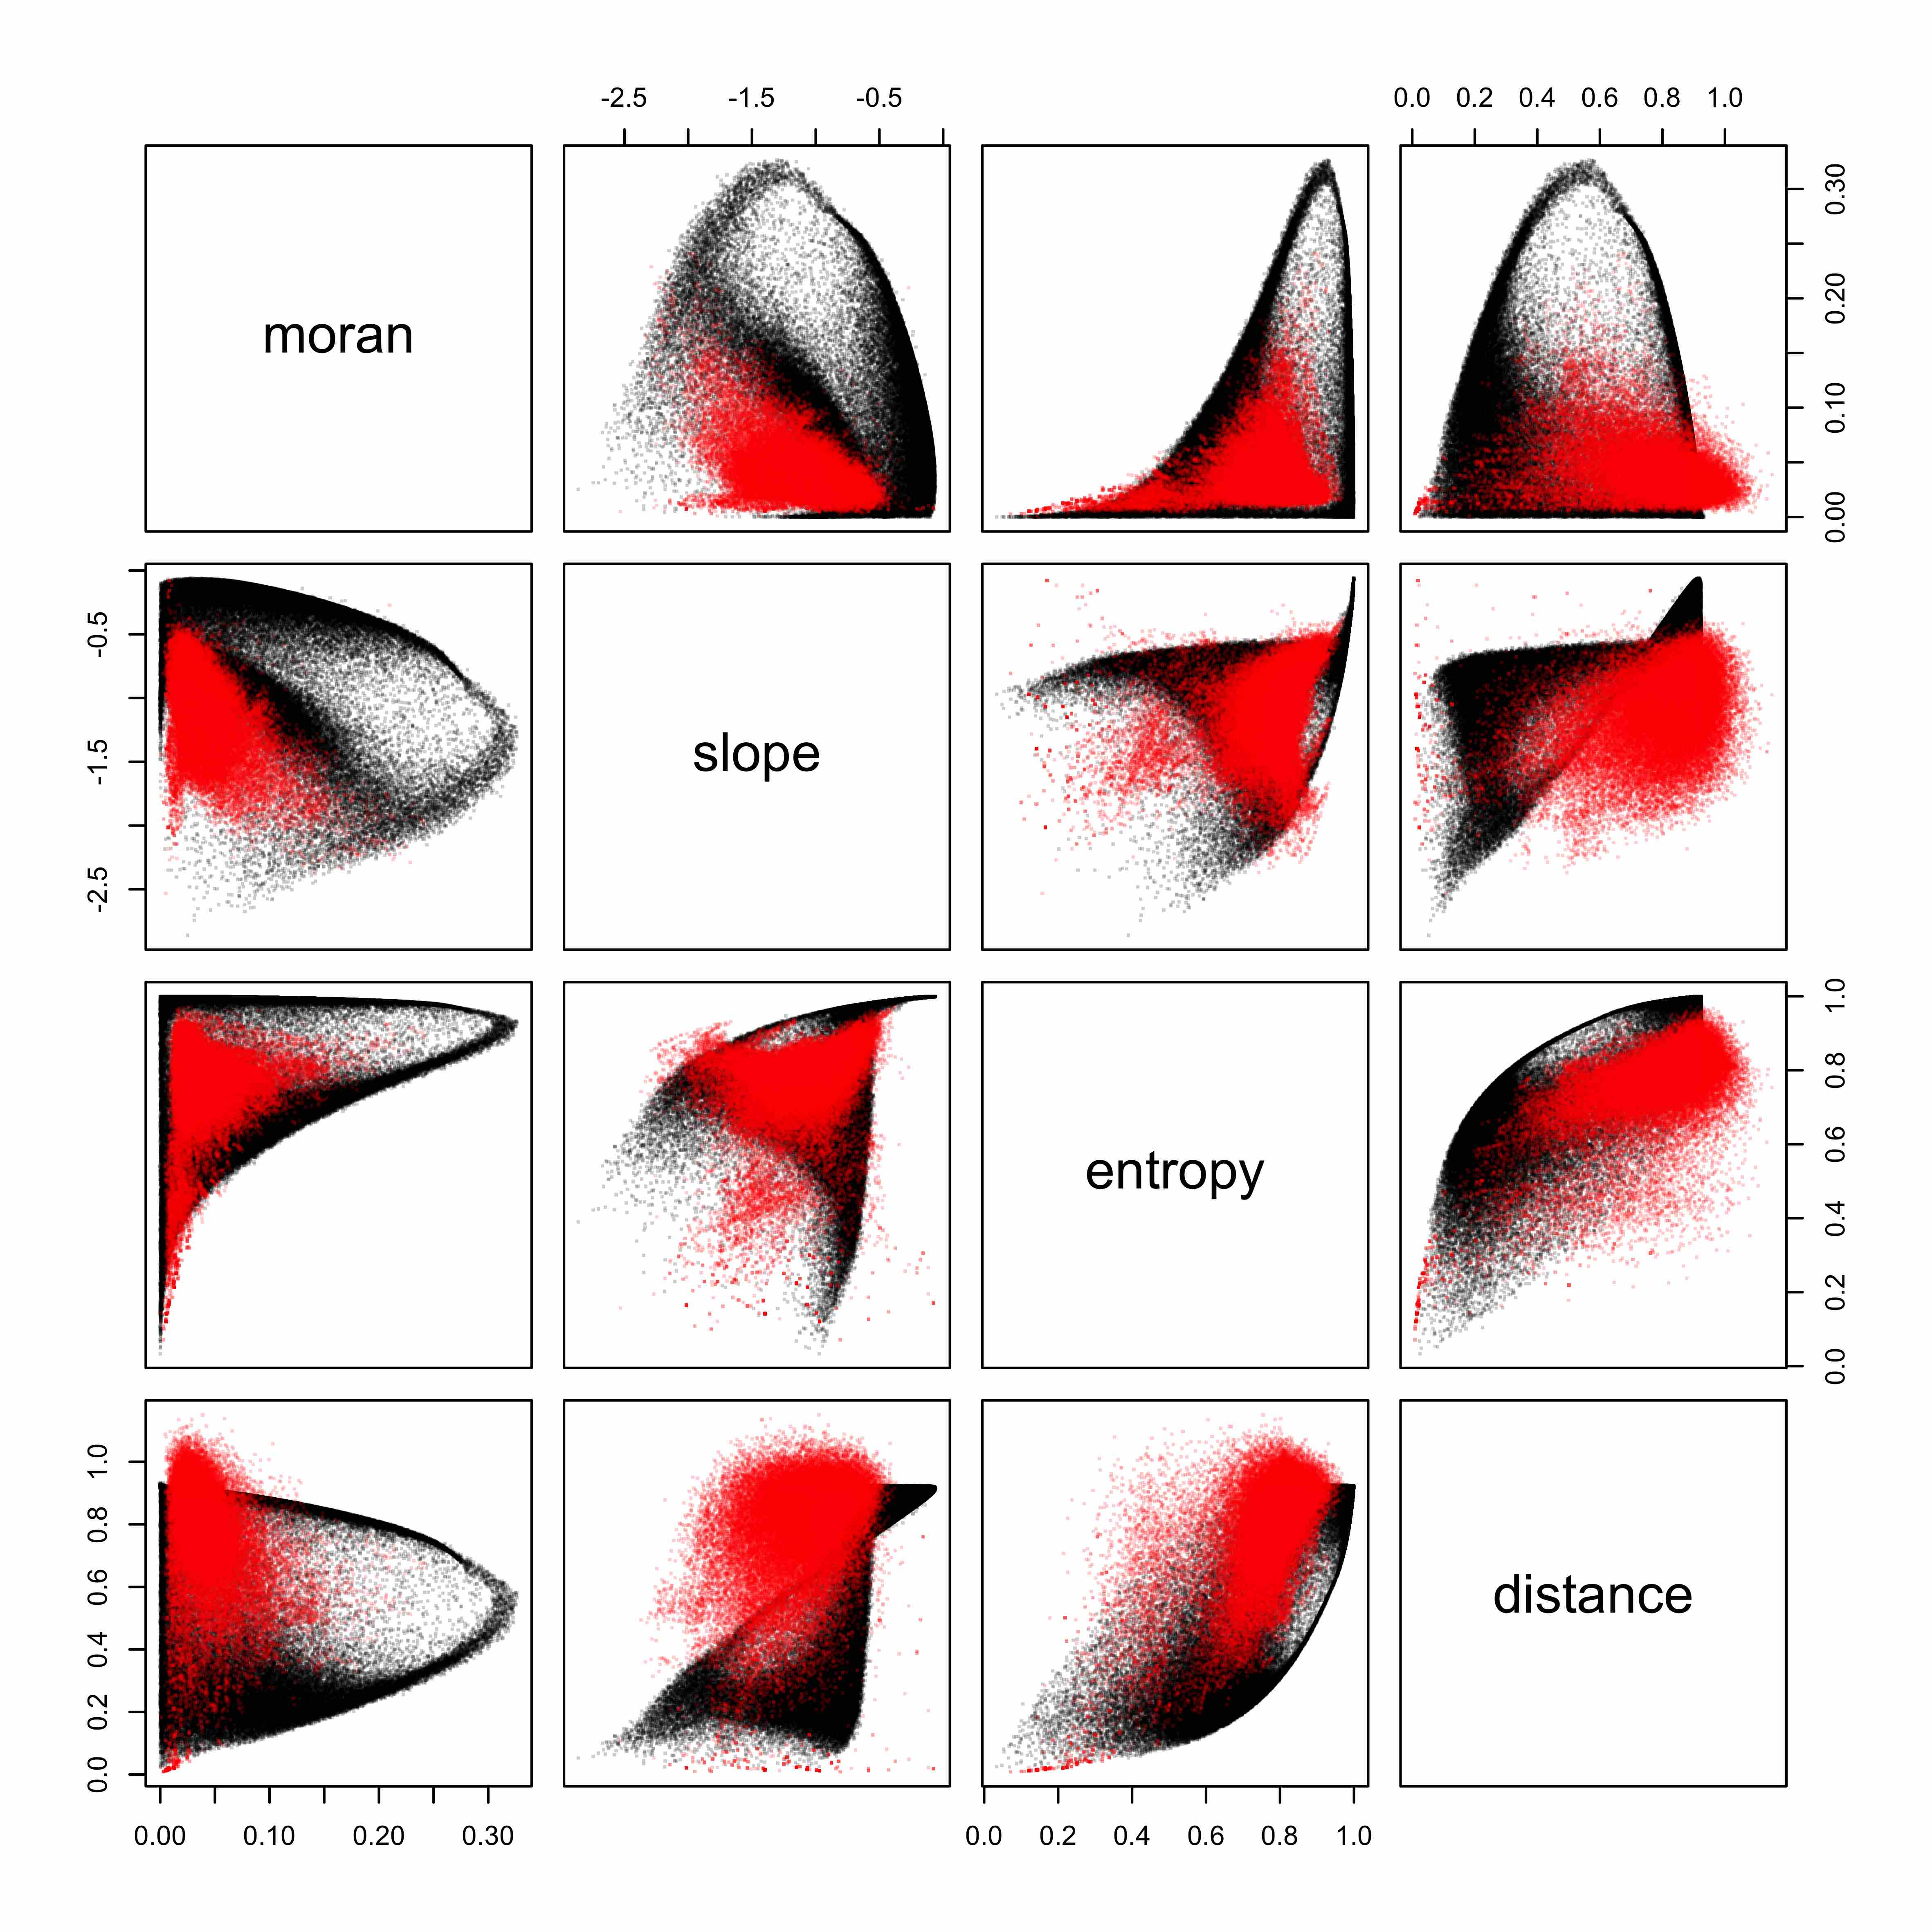
\includegraphics[width=\textwidth]{figuresraw/scatter}
\caption{Scatterplots of indicators distribution in an hypercube of the parameter space. Red points correspond to real data.}
\label{fig:densityscatter}
\end{figure}
%%%%%%%%%%%%%



\subsection*{Indicators Behavior}

% full plots behavior



%%%%%%%%%%%%%%%%%%%%
\begin{figure}
\centering
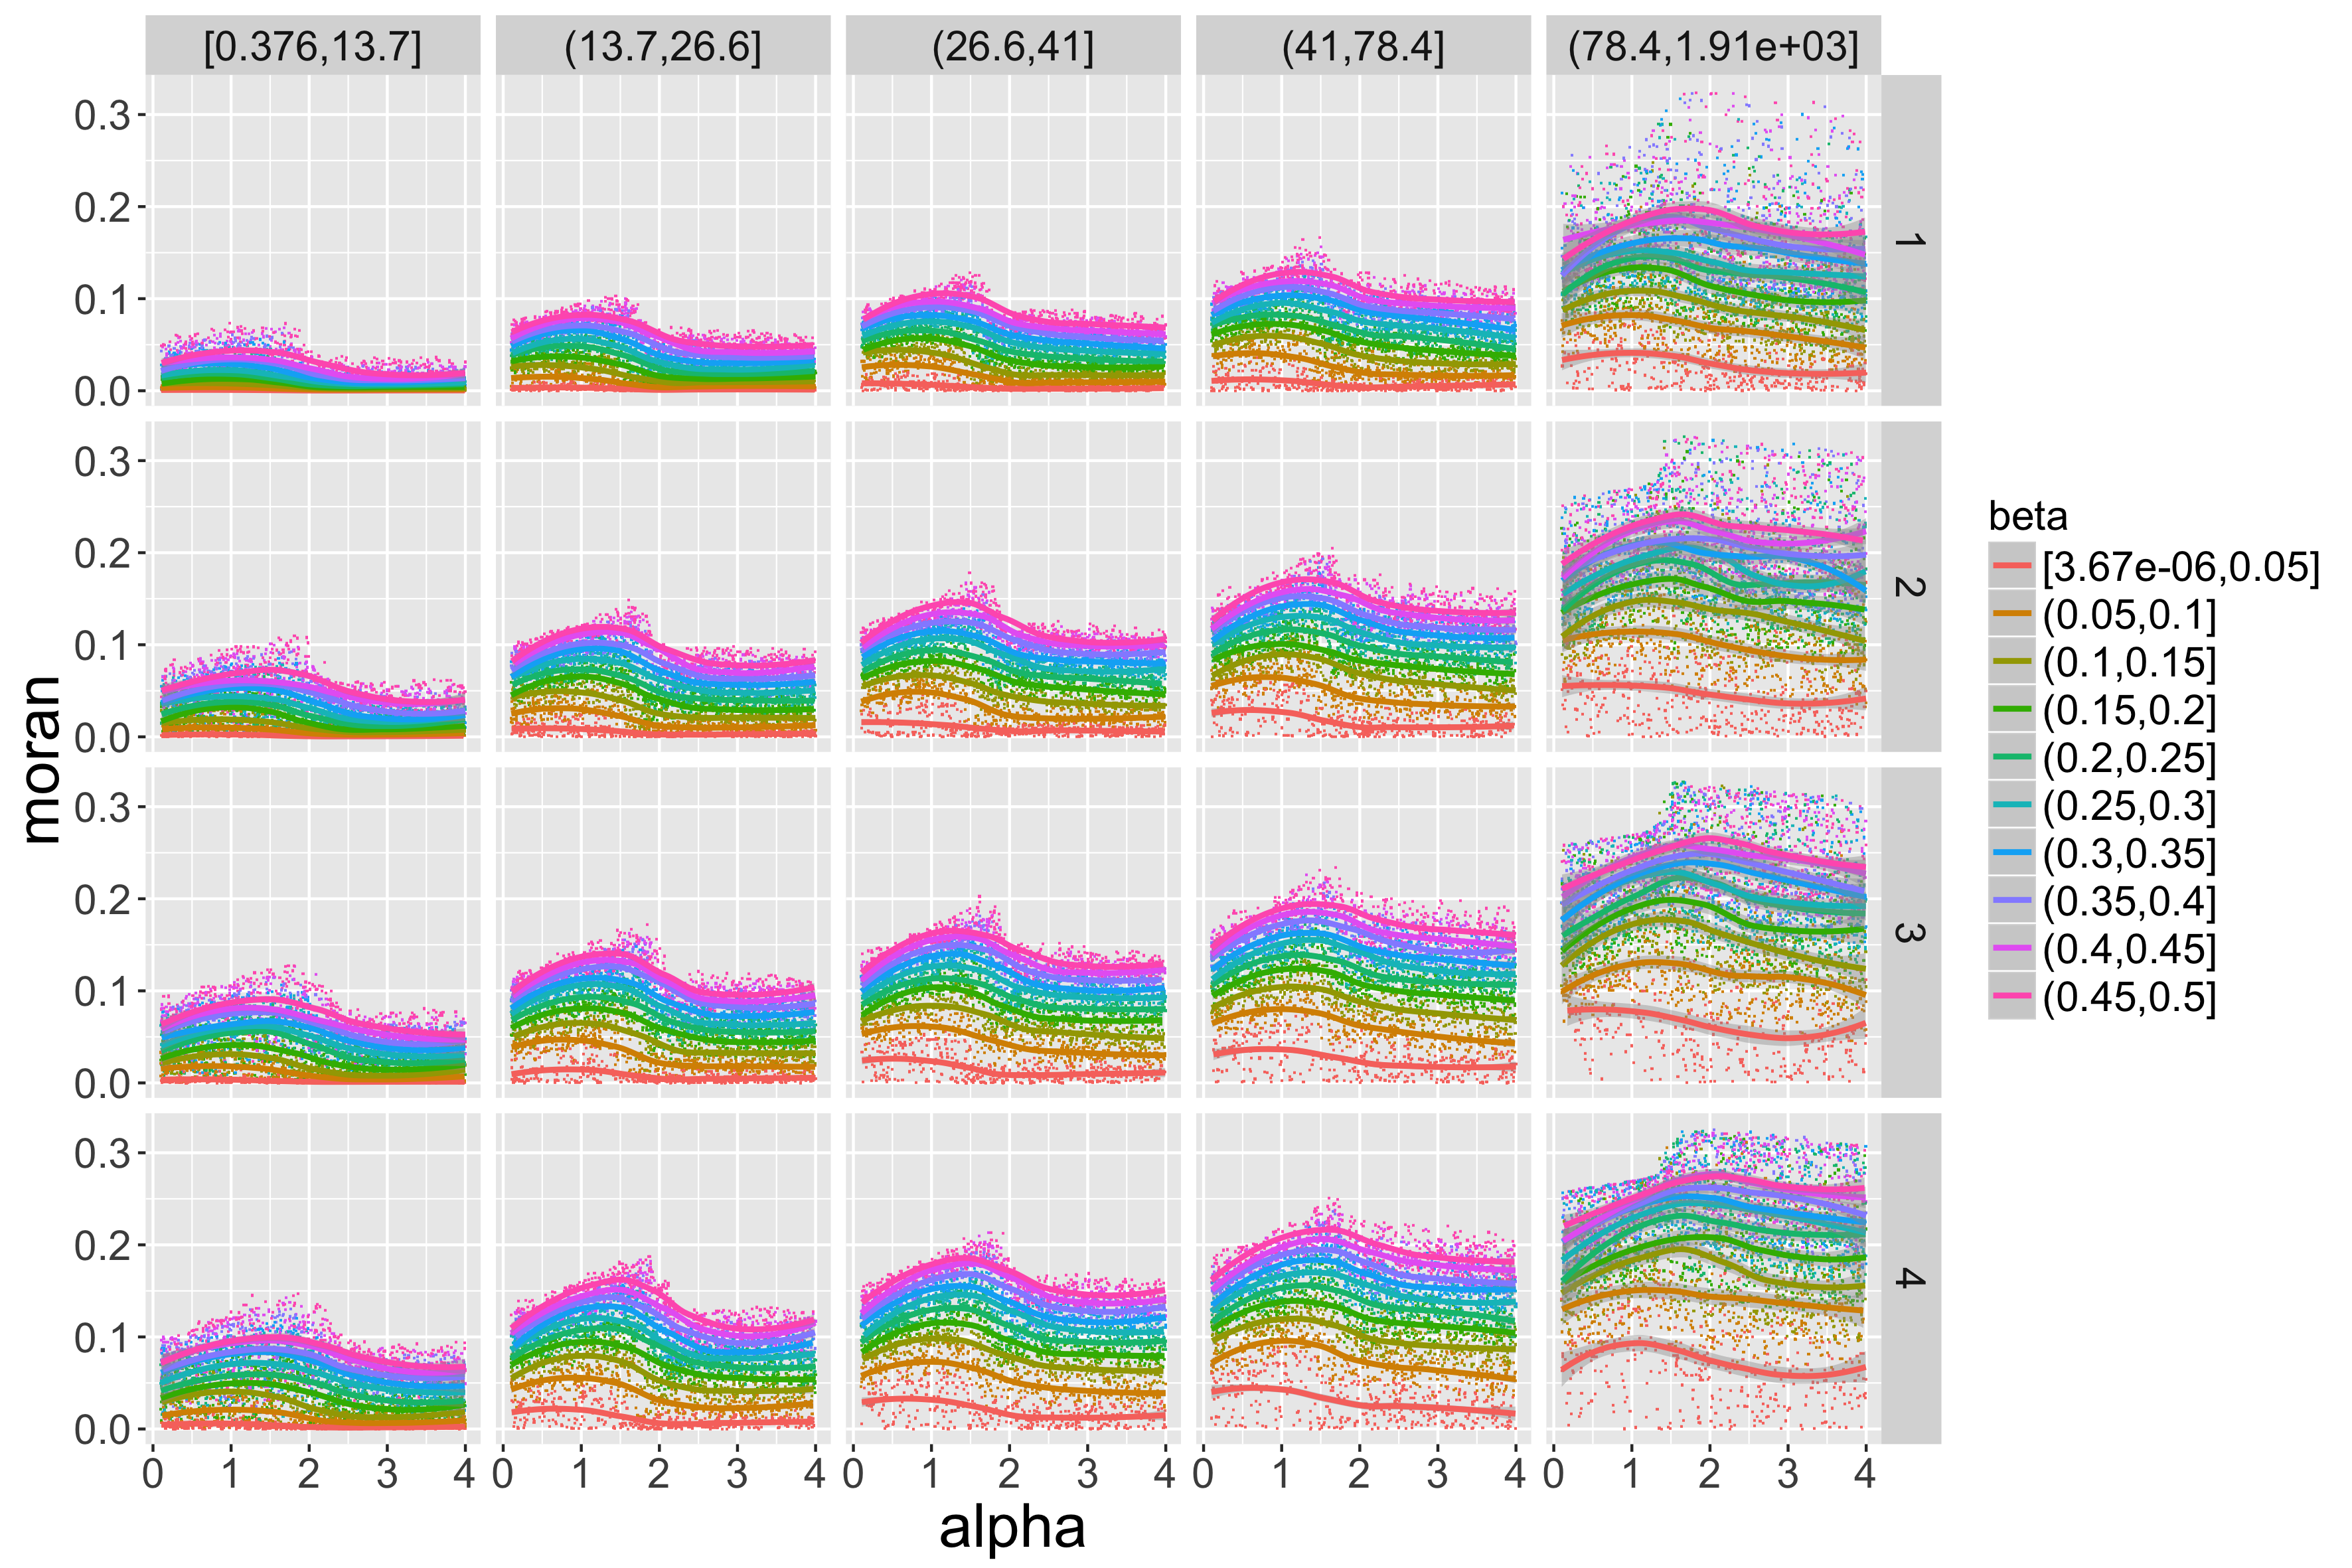
\includegraphics[width=\textwidth]{figuresraw/moran_alpha}
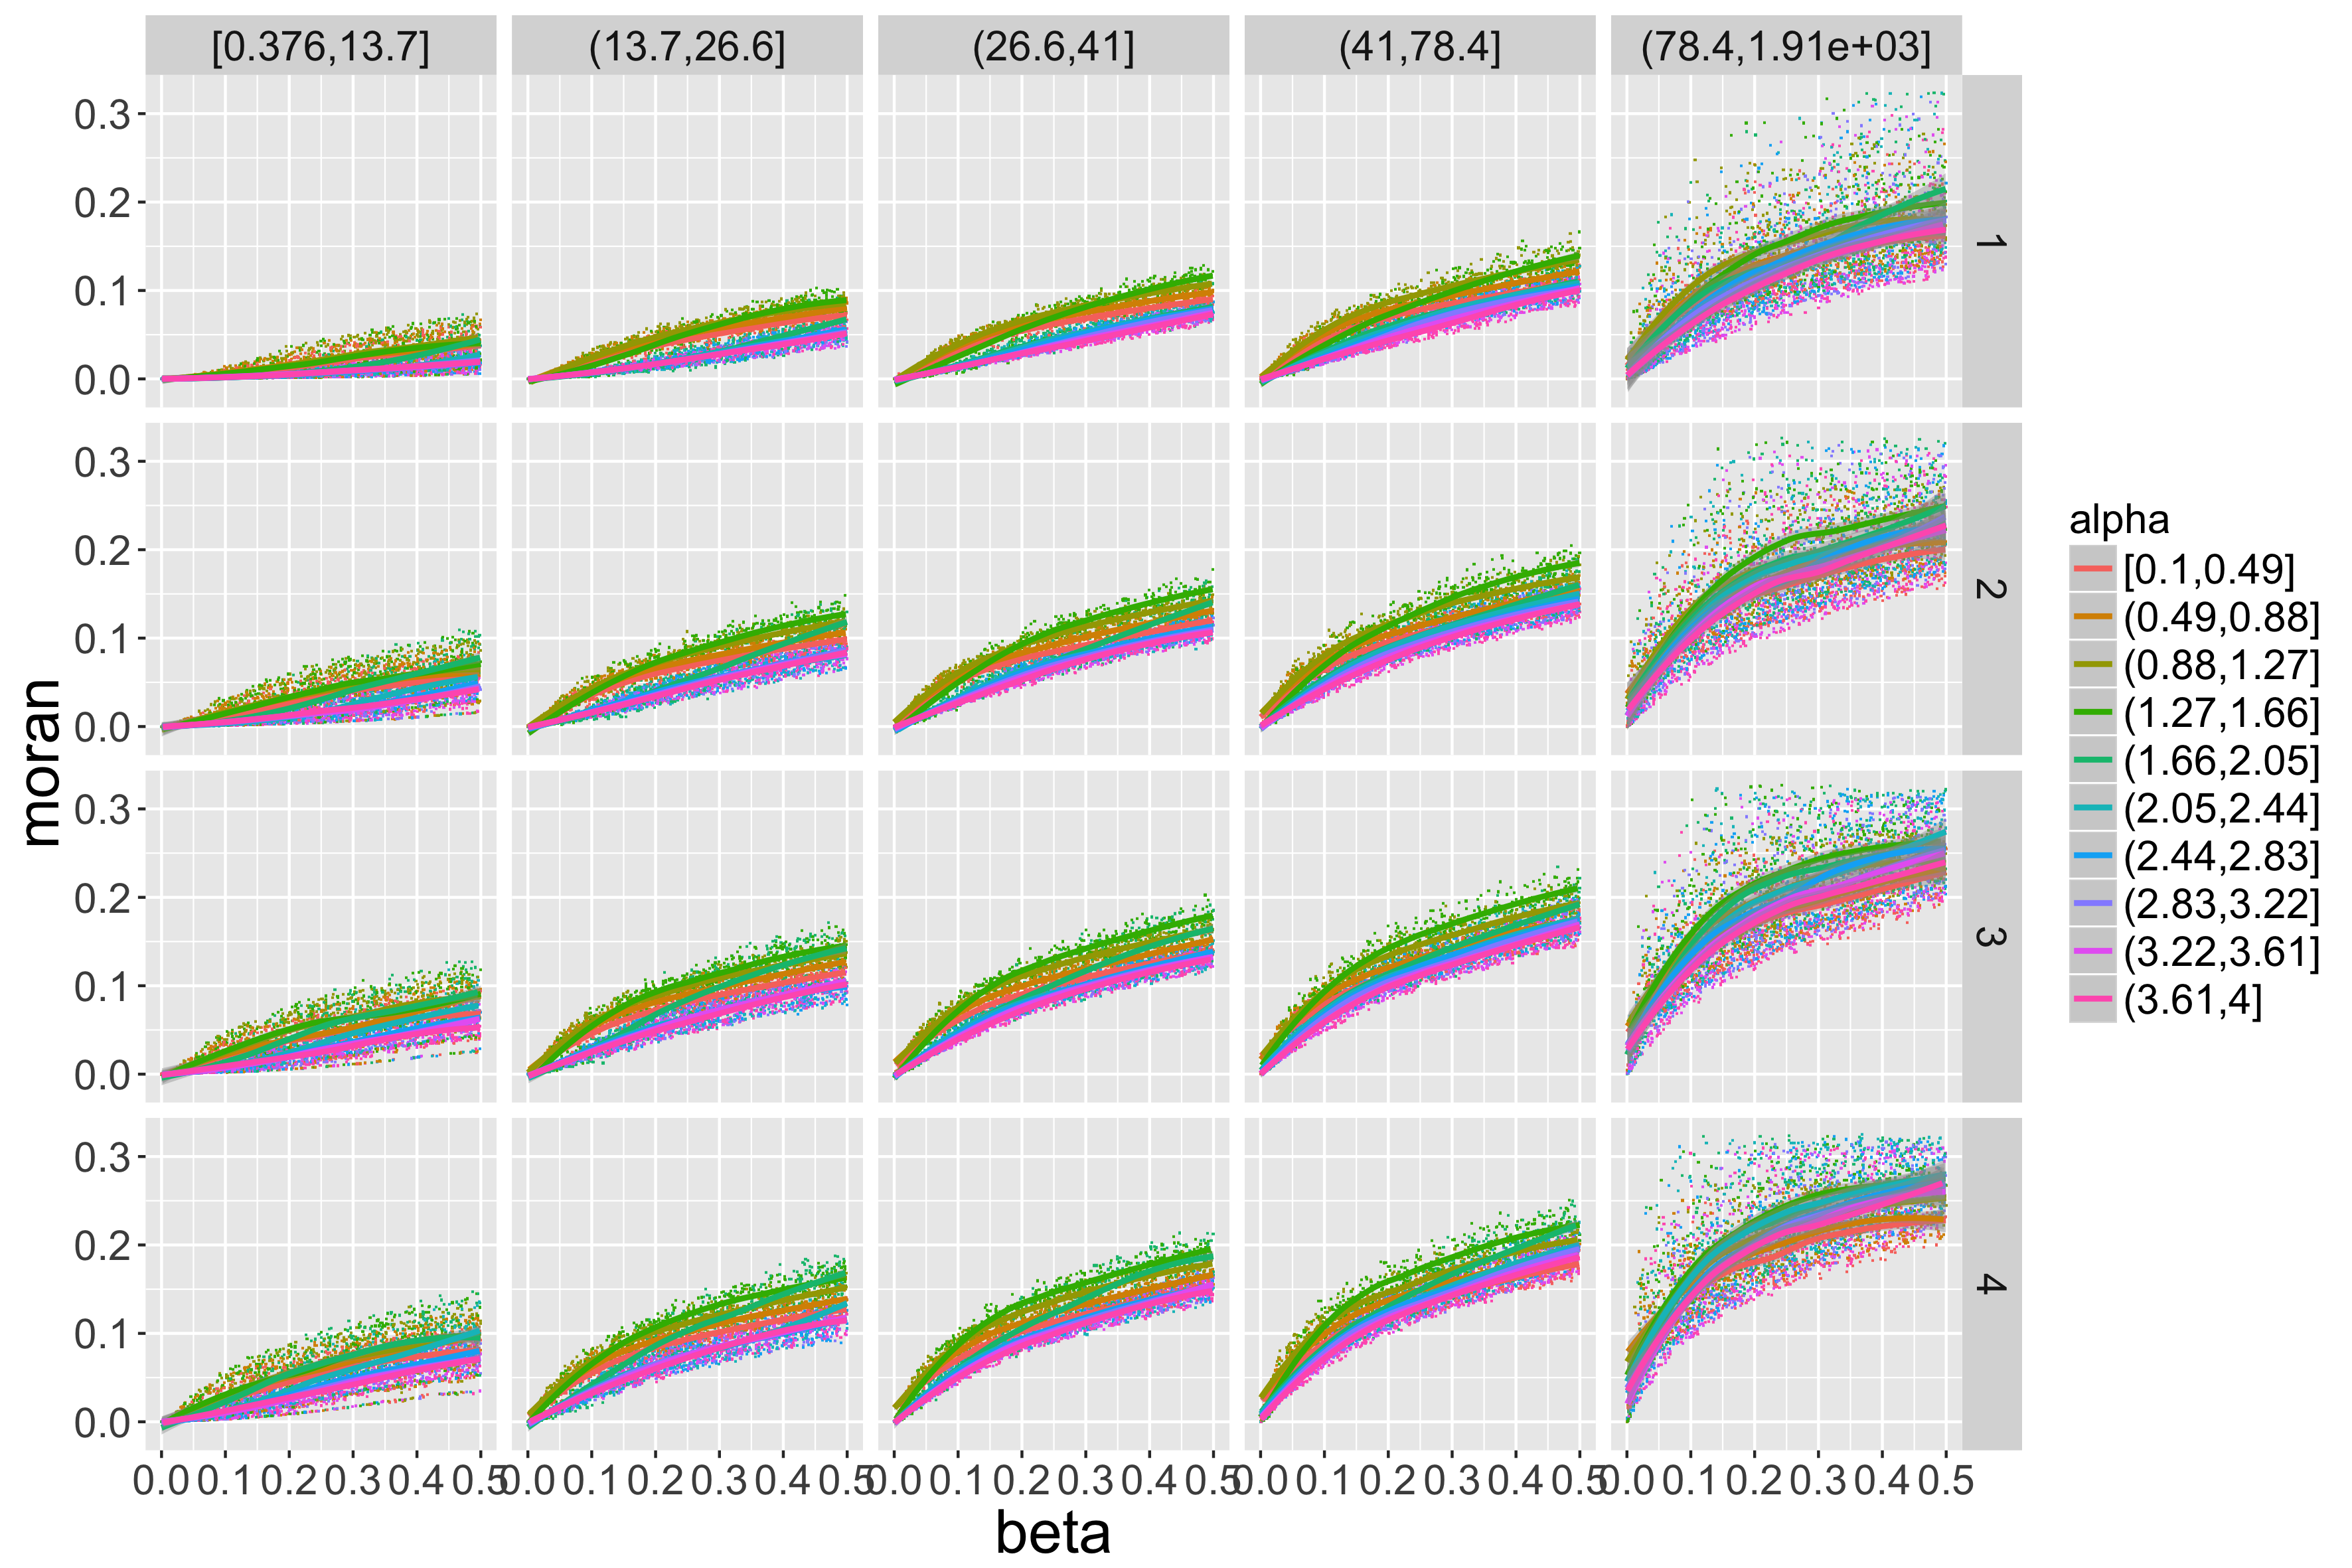
\includegraphics[width=\textwidth]{figuresraw/moran_beta}
\caption{Moran index as a function of $\alpha$ (Top) and $\beta$ (Bottom) for varying $\beta$ (resp. $\alpha$) given by color, and varying $n_d$ (row) and $N_G$}
\label{}
\end{figure}
%%%%%%%%%%%%%%%%%%%%

%%%%%%%%%%%%%%%%%%%%
\begin{figure}
\centering
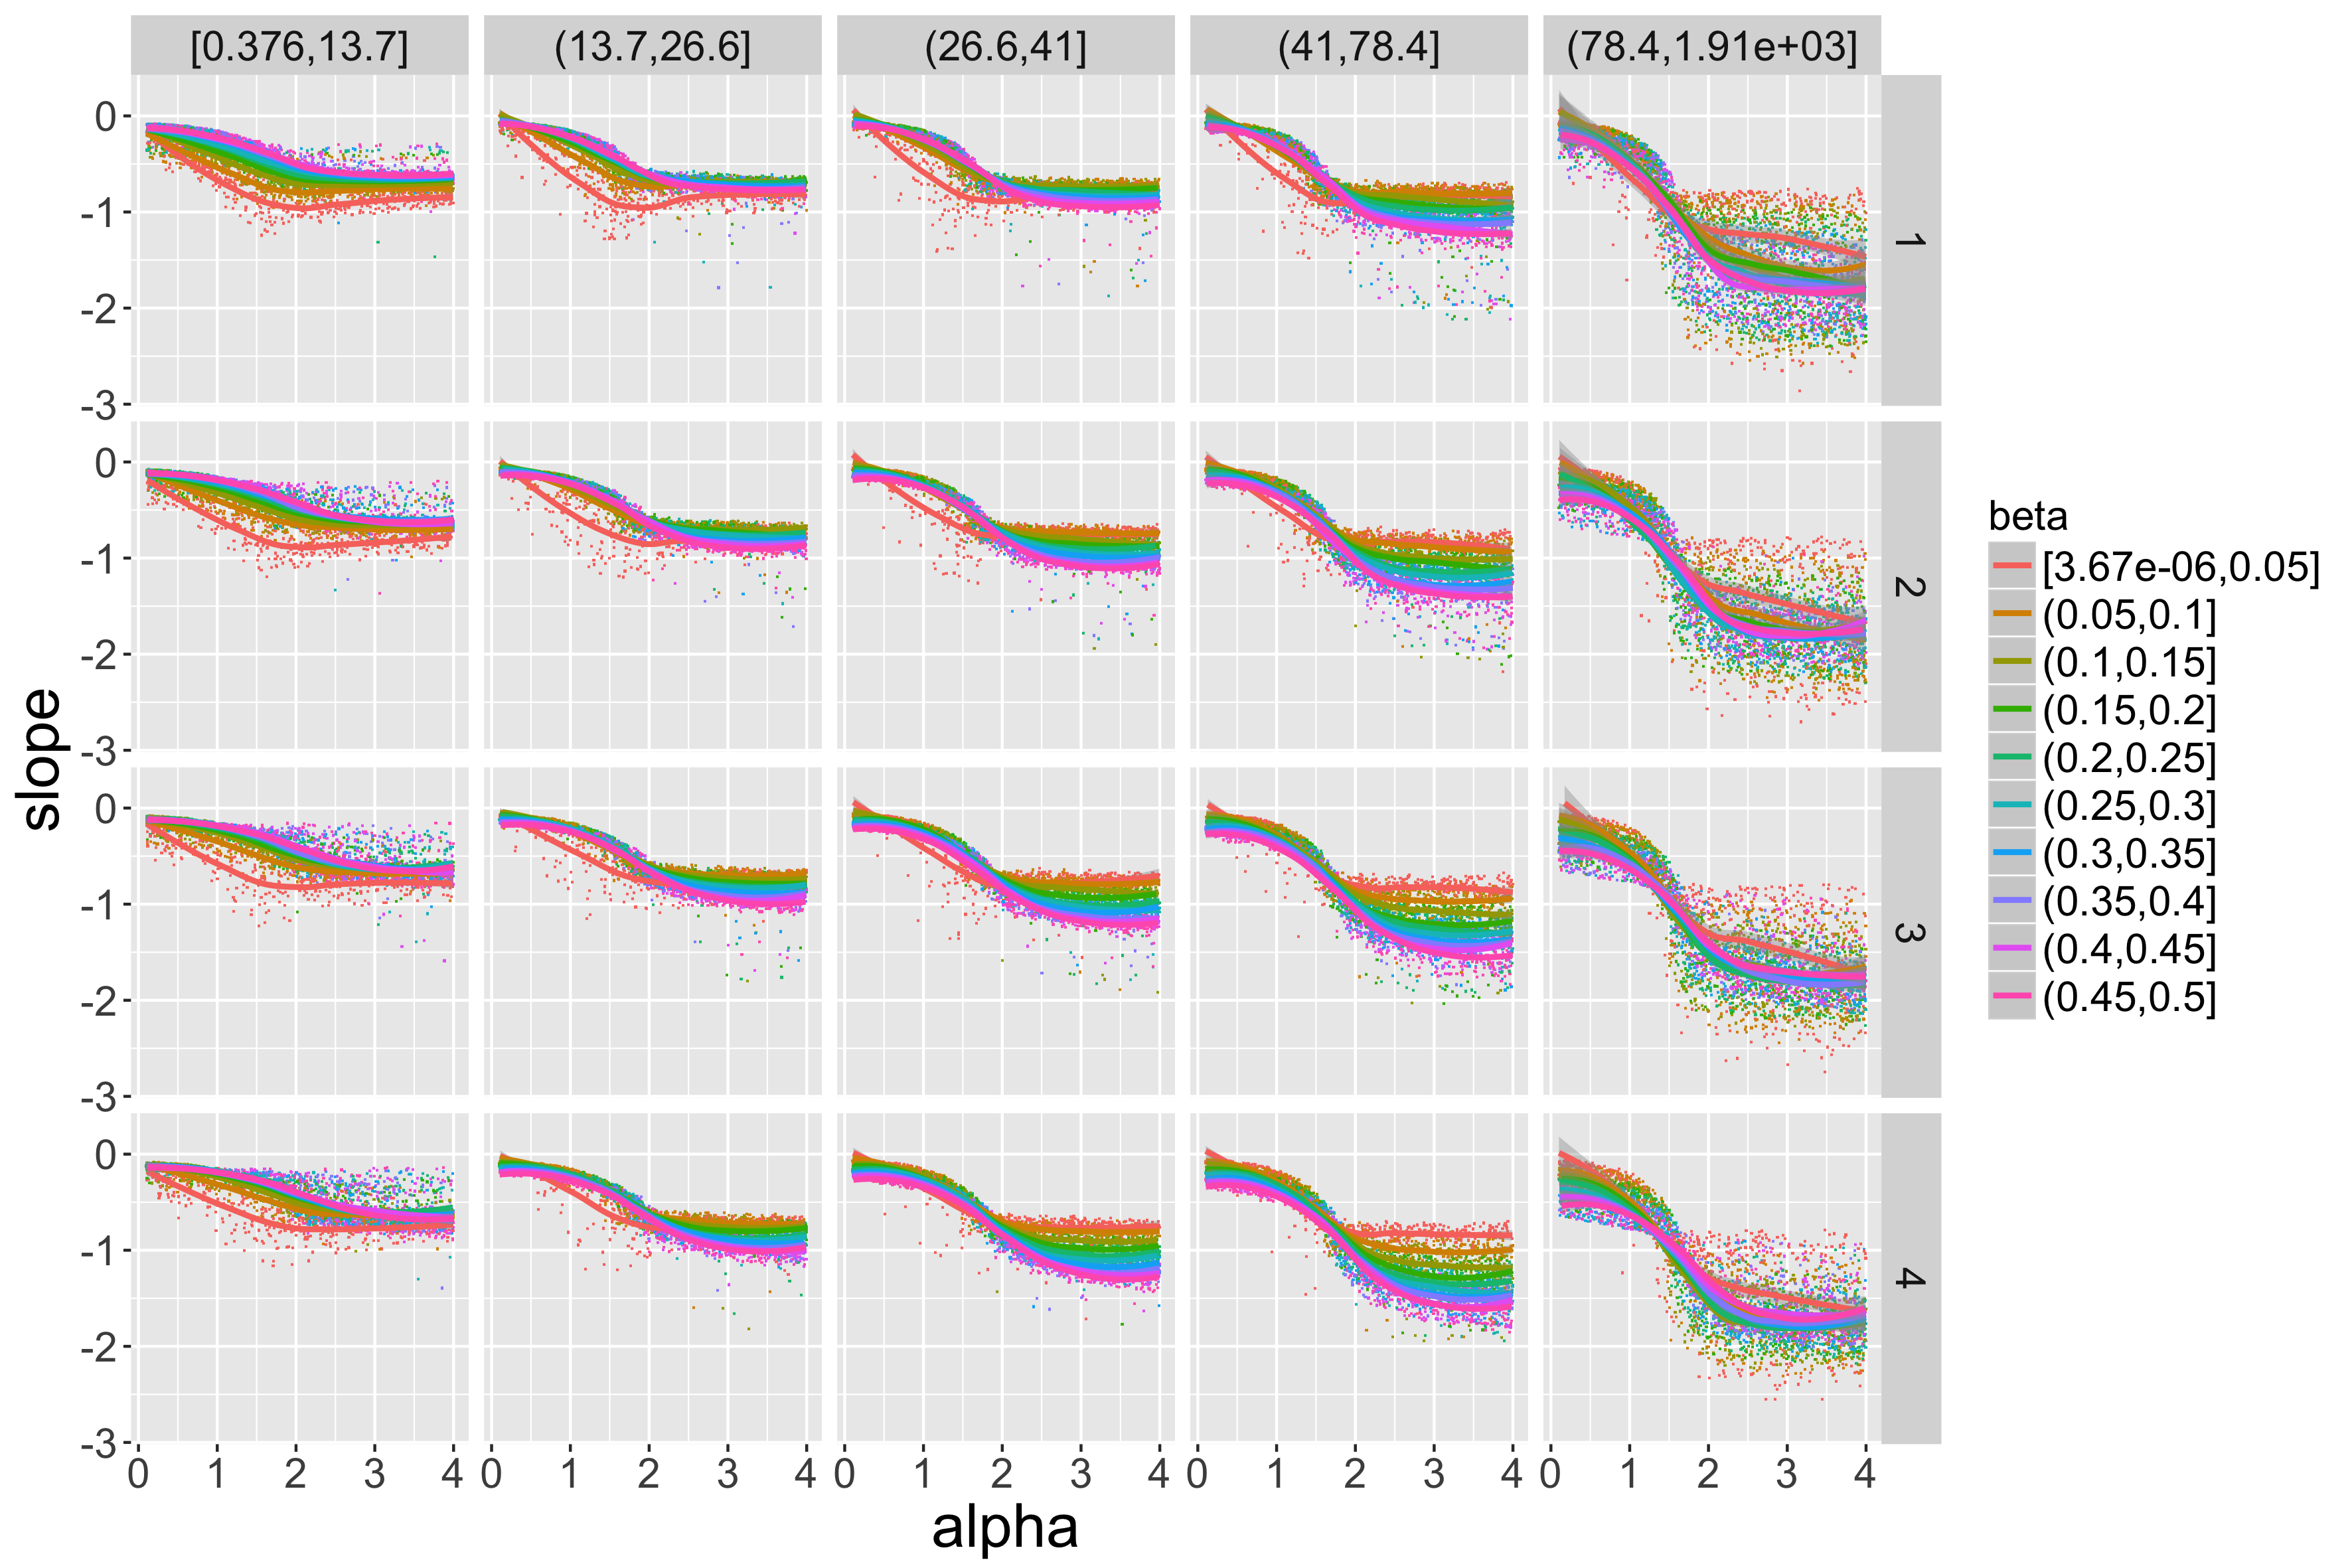
\includegraphics[width=\textwidth]{figuresraw/slope_alpha}
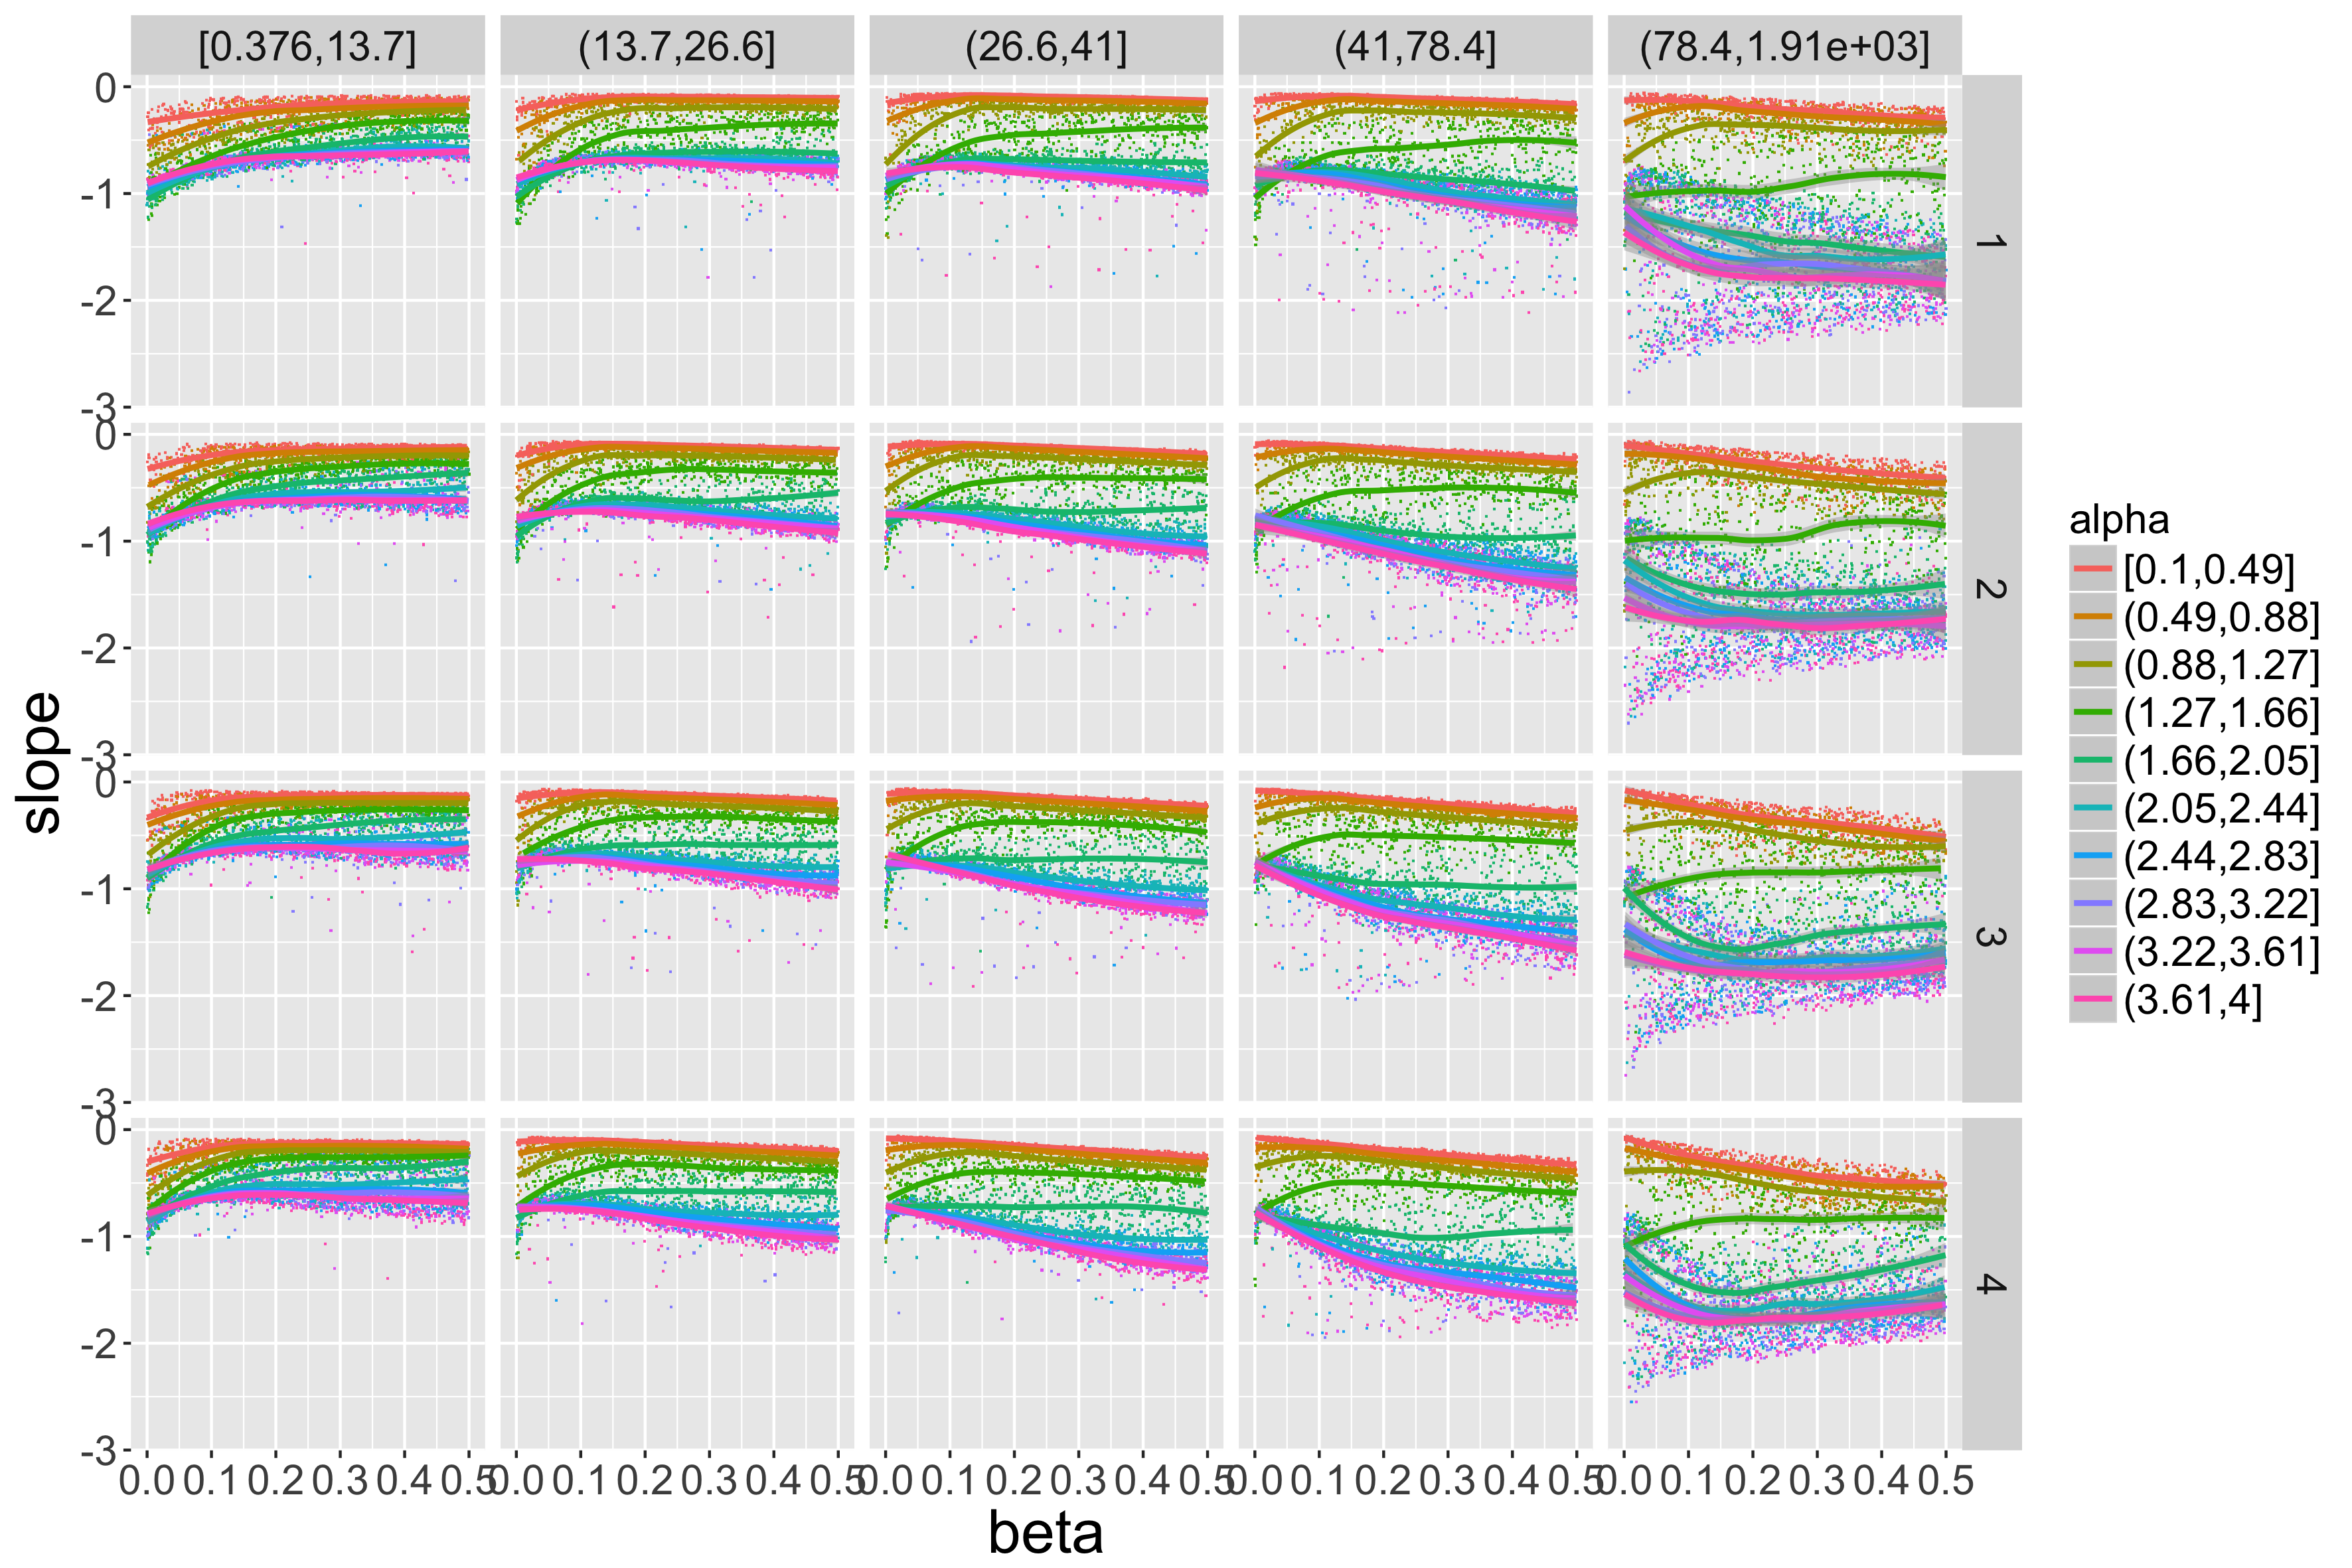
\includegraphics[width=\textwidth]{figuresraw/slope_beta}
\caption{}
\label{}
\end{figure}
%%%%%%%%%%%%%%%%%%%%


%%%%%%%%%%%%%%%%%%%%
\begin{figure}
\centering
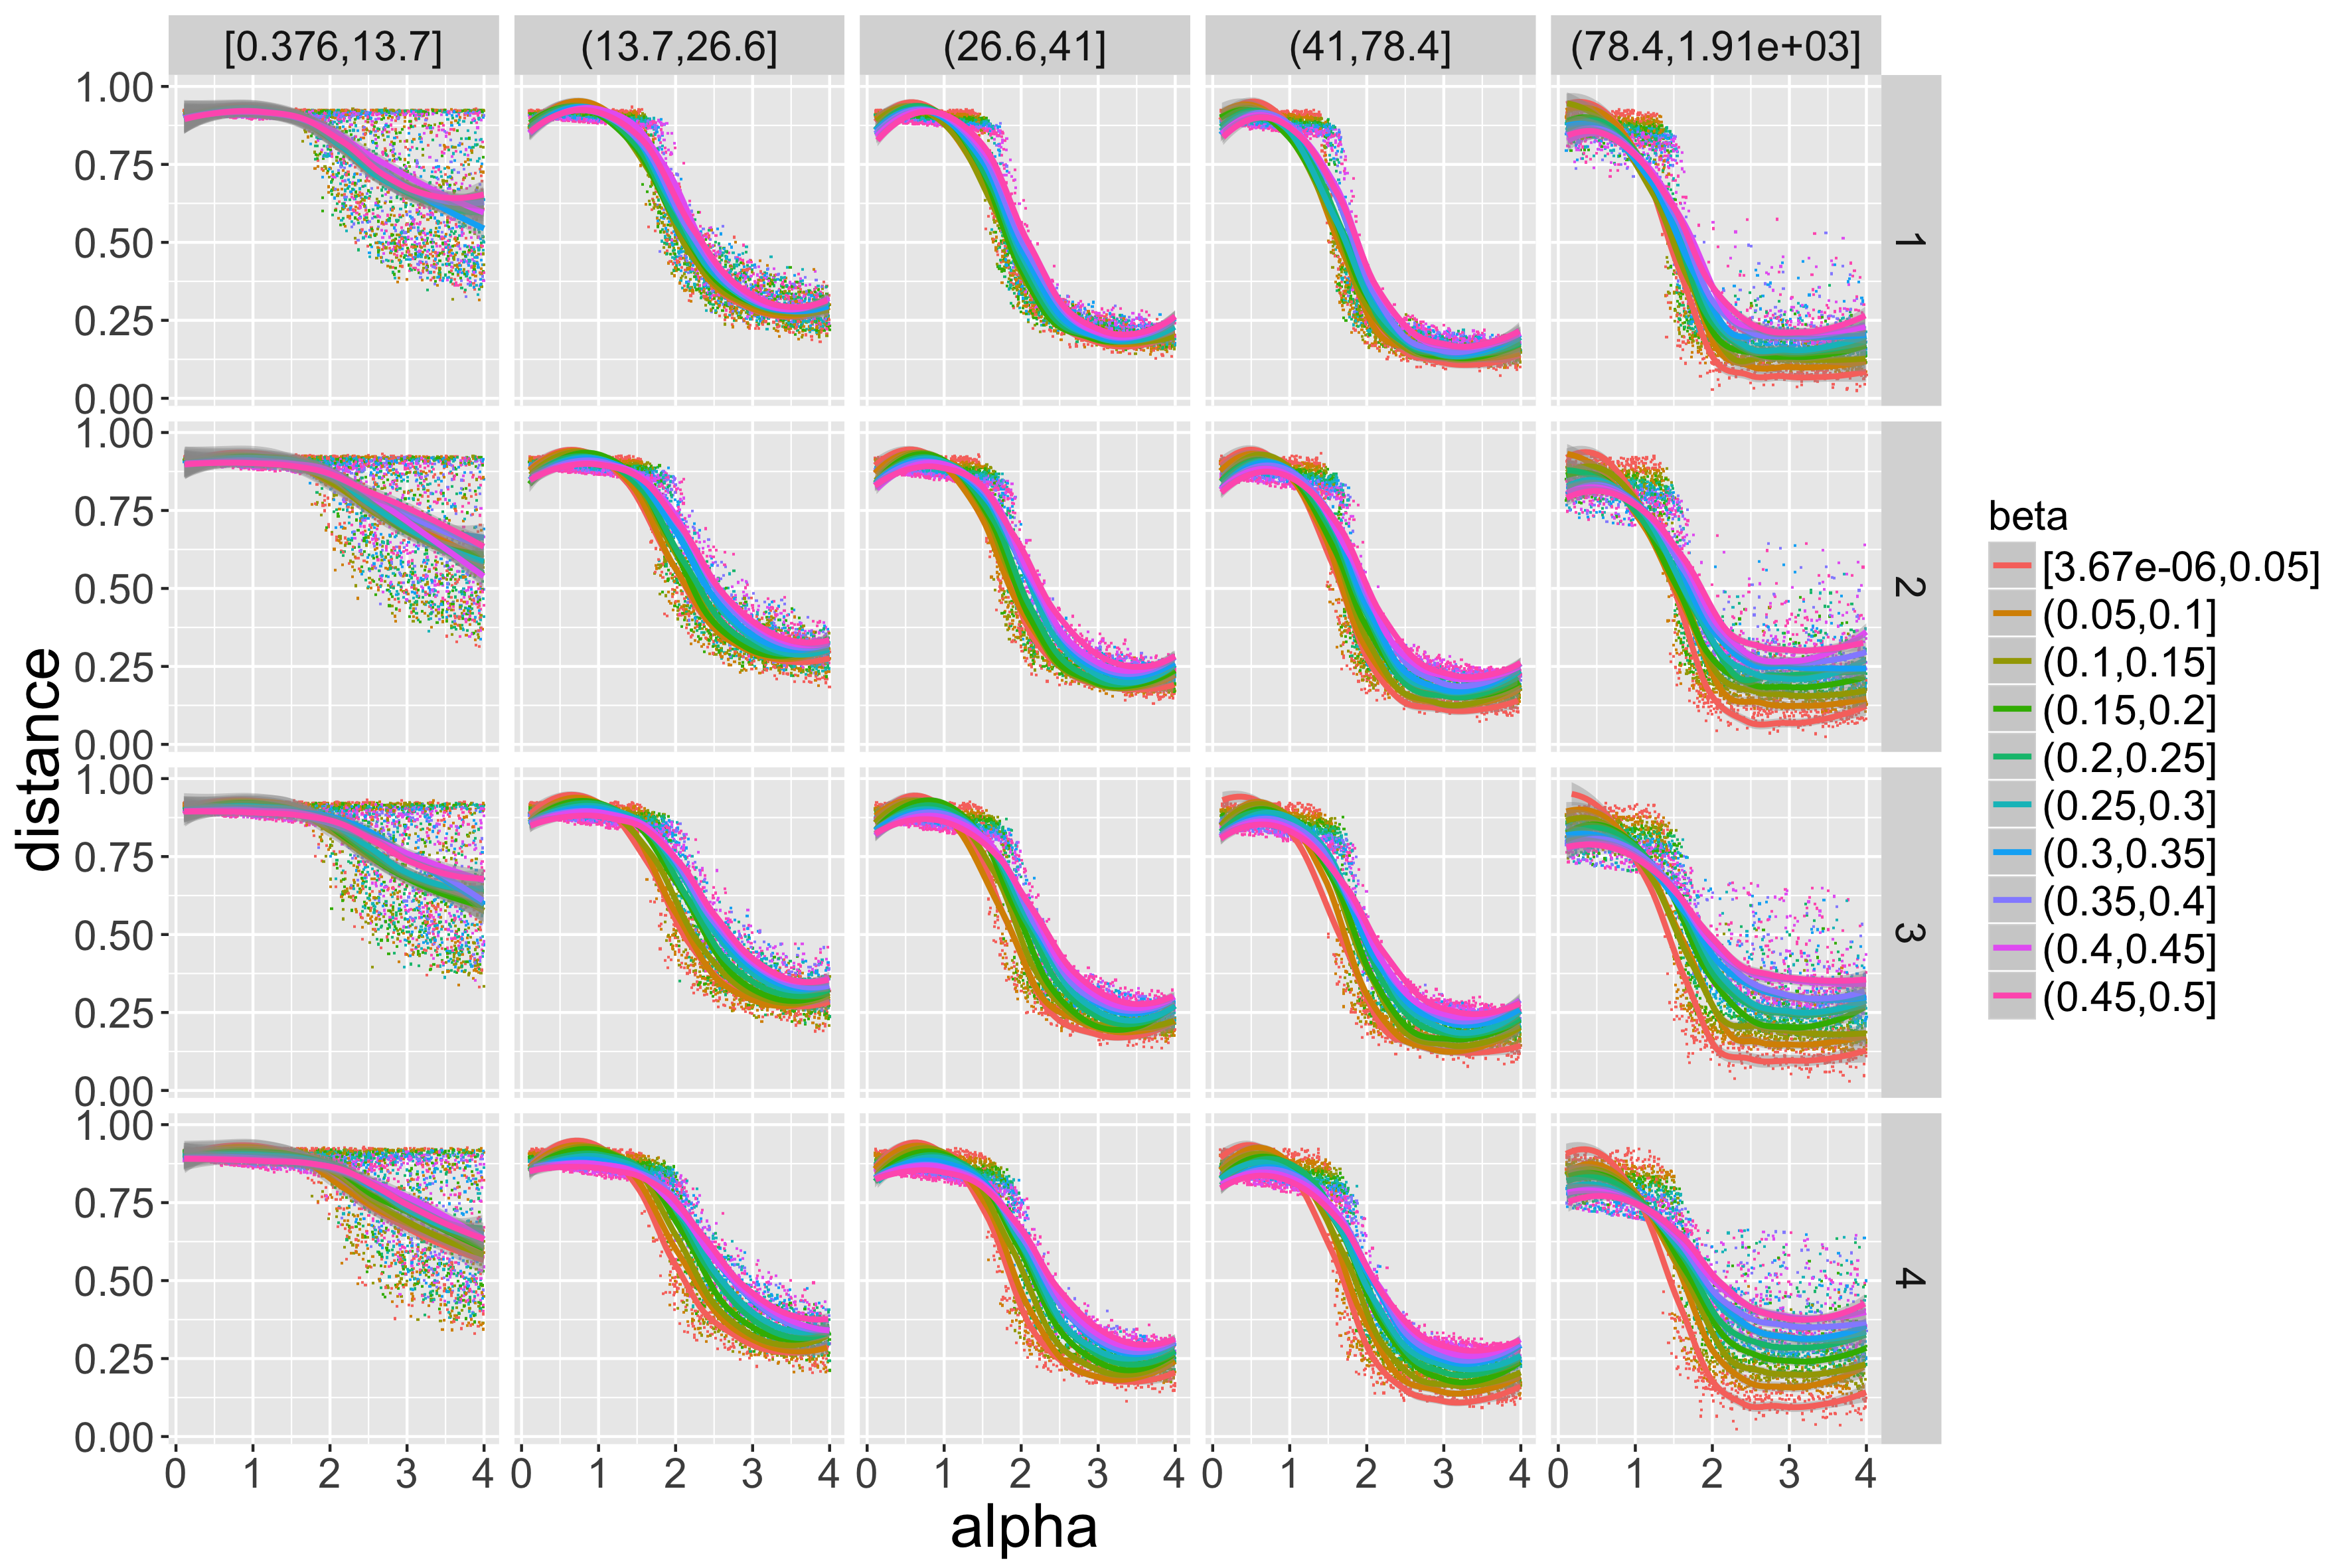
\includegraphics[width=\textwidth]{figuresraw/distance_alpha}
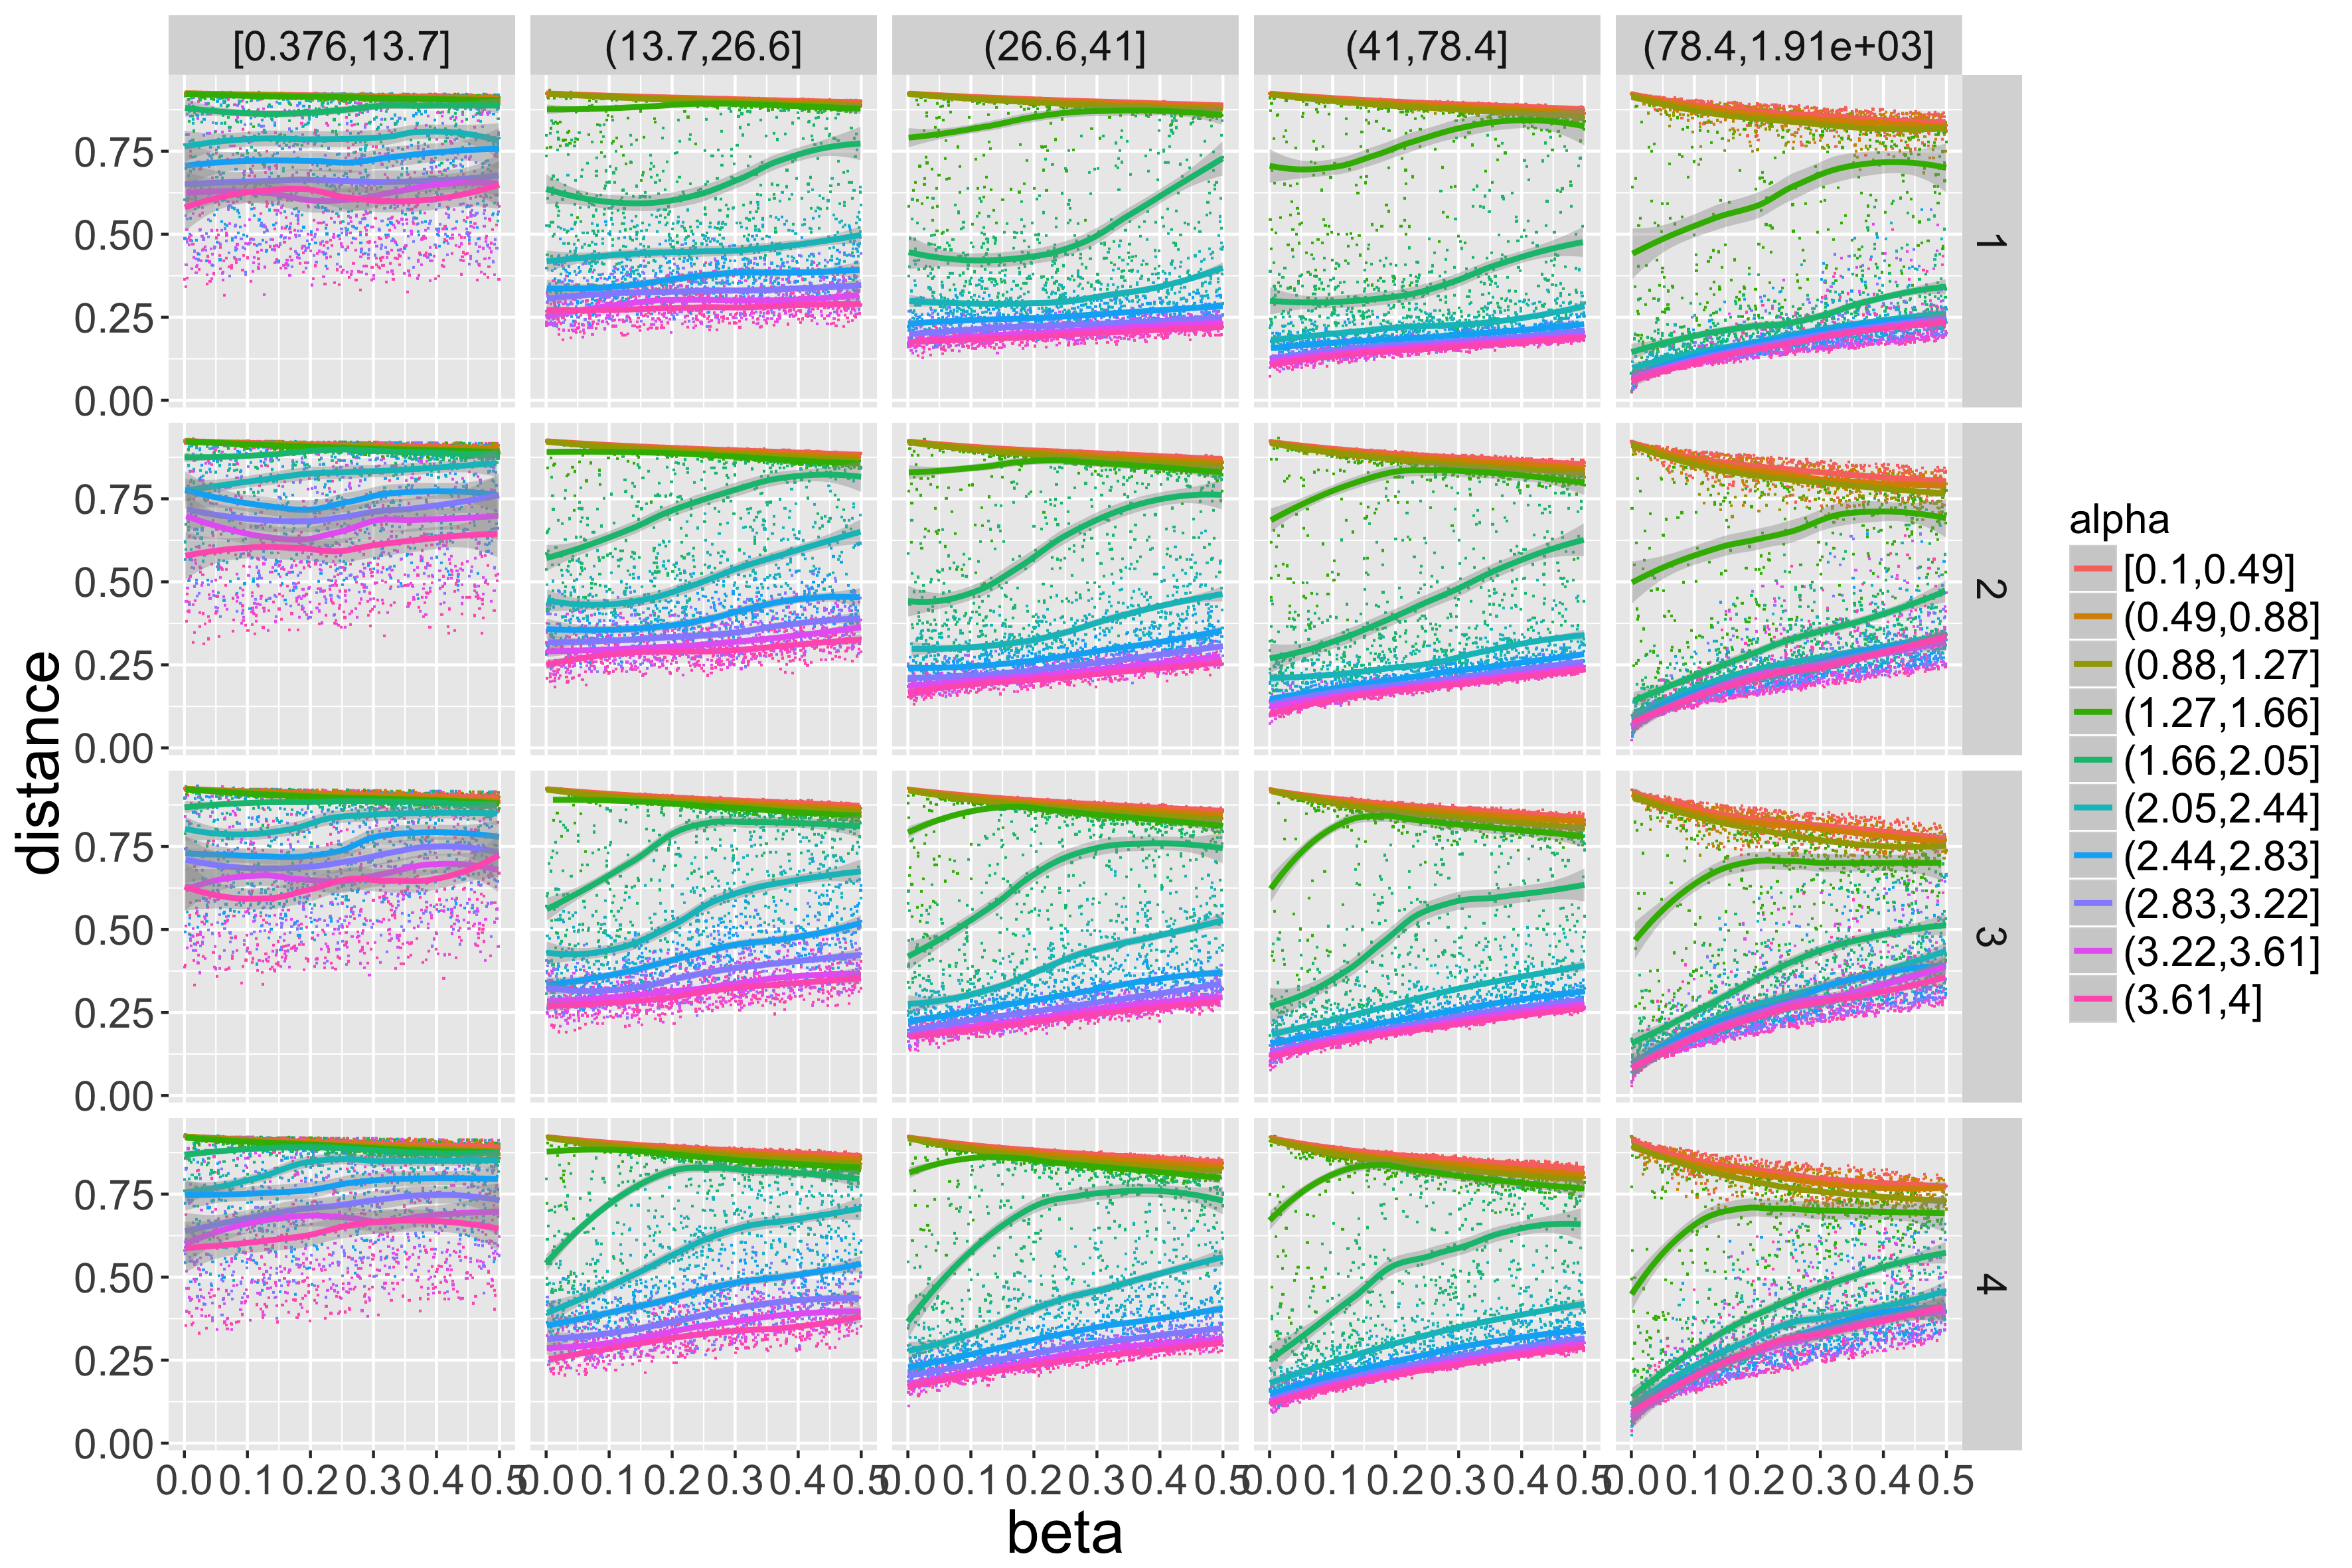
\includegraphics[width=\textwidth]{figuresraw/distance_beta}
\caption{}
\label{}
\end{figure}
%%%%%%%%%%%%%%%%%%%%

%%%%%%%%%%%%%%%%%%%%
\begin{figure}
\centering
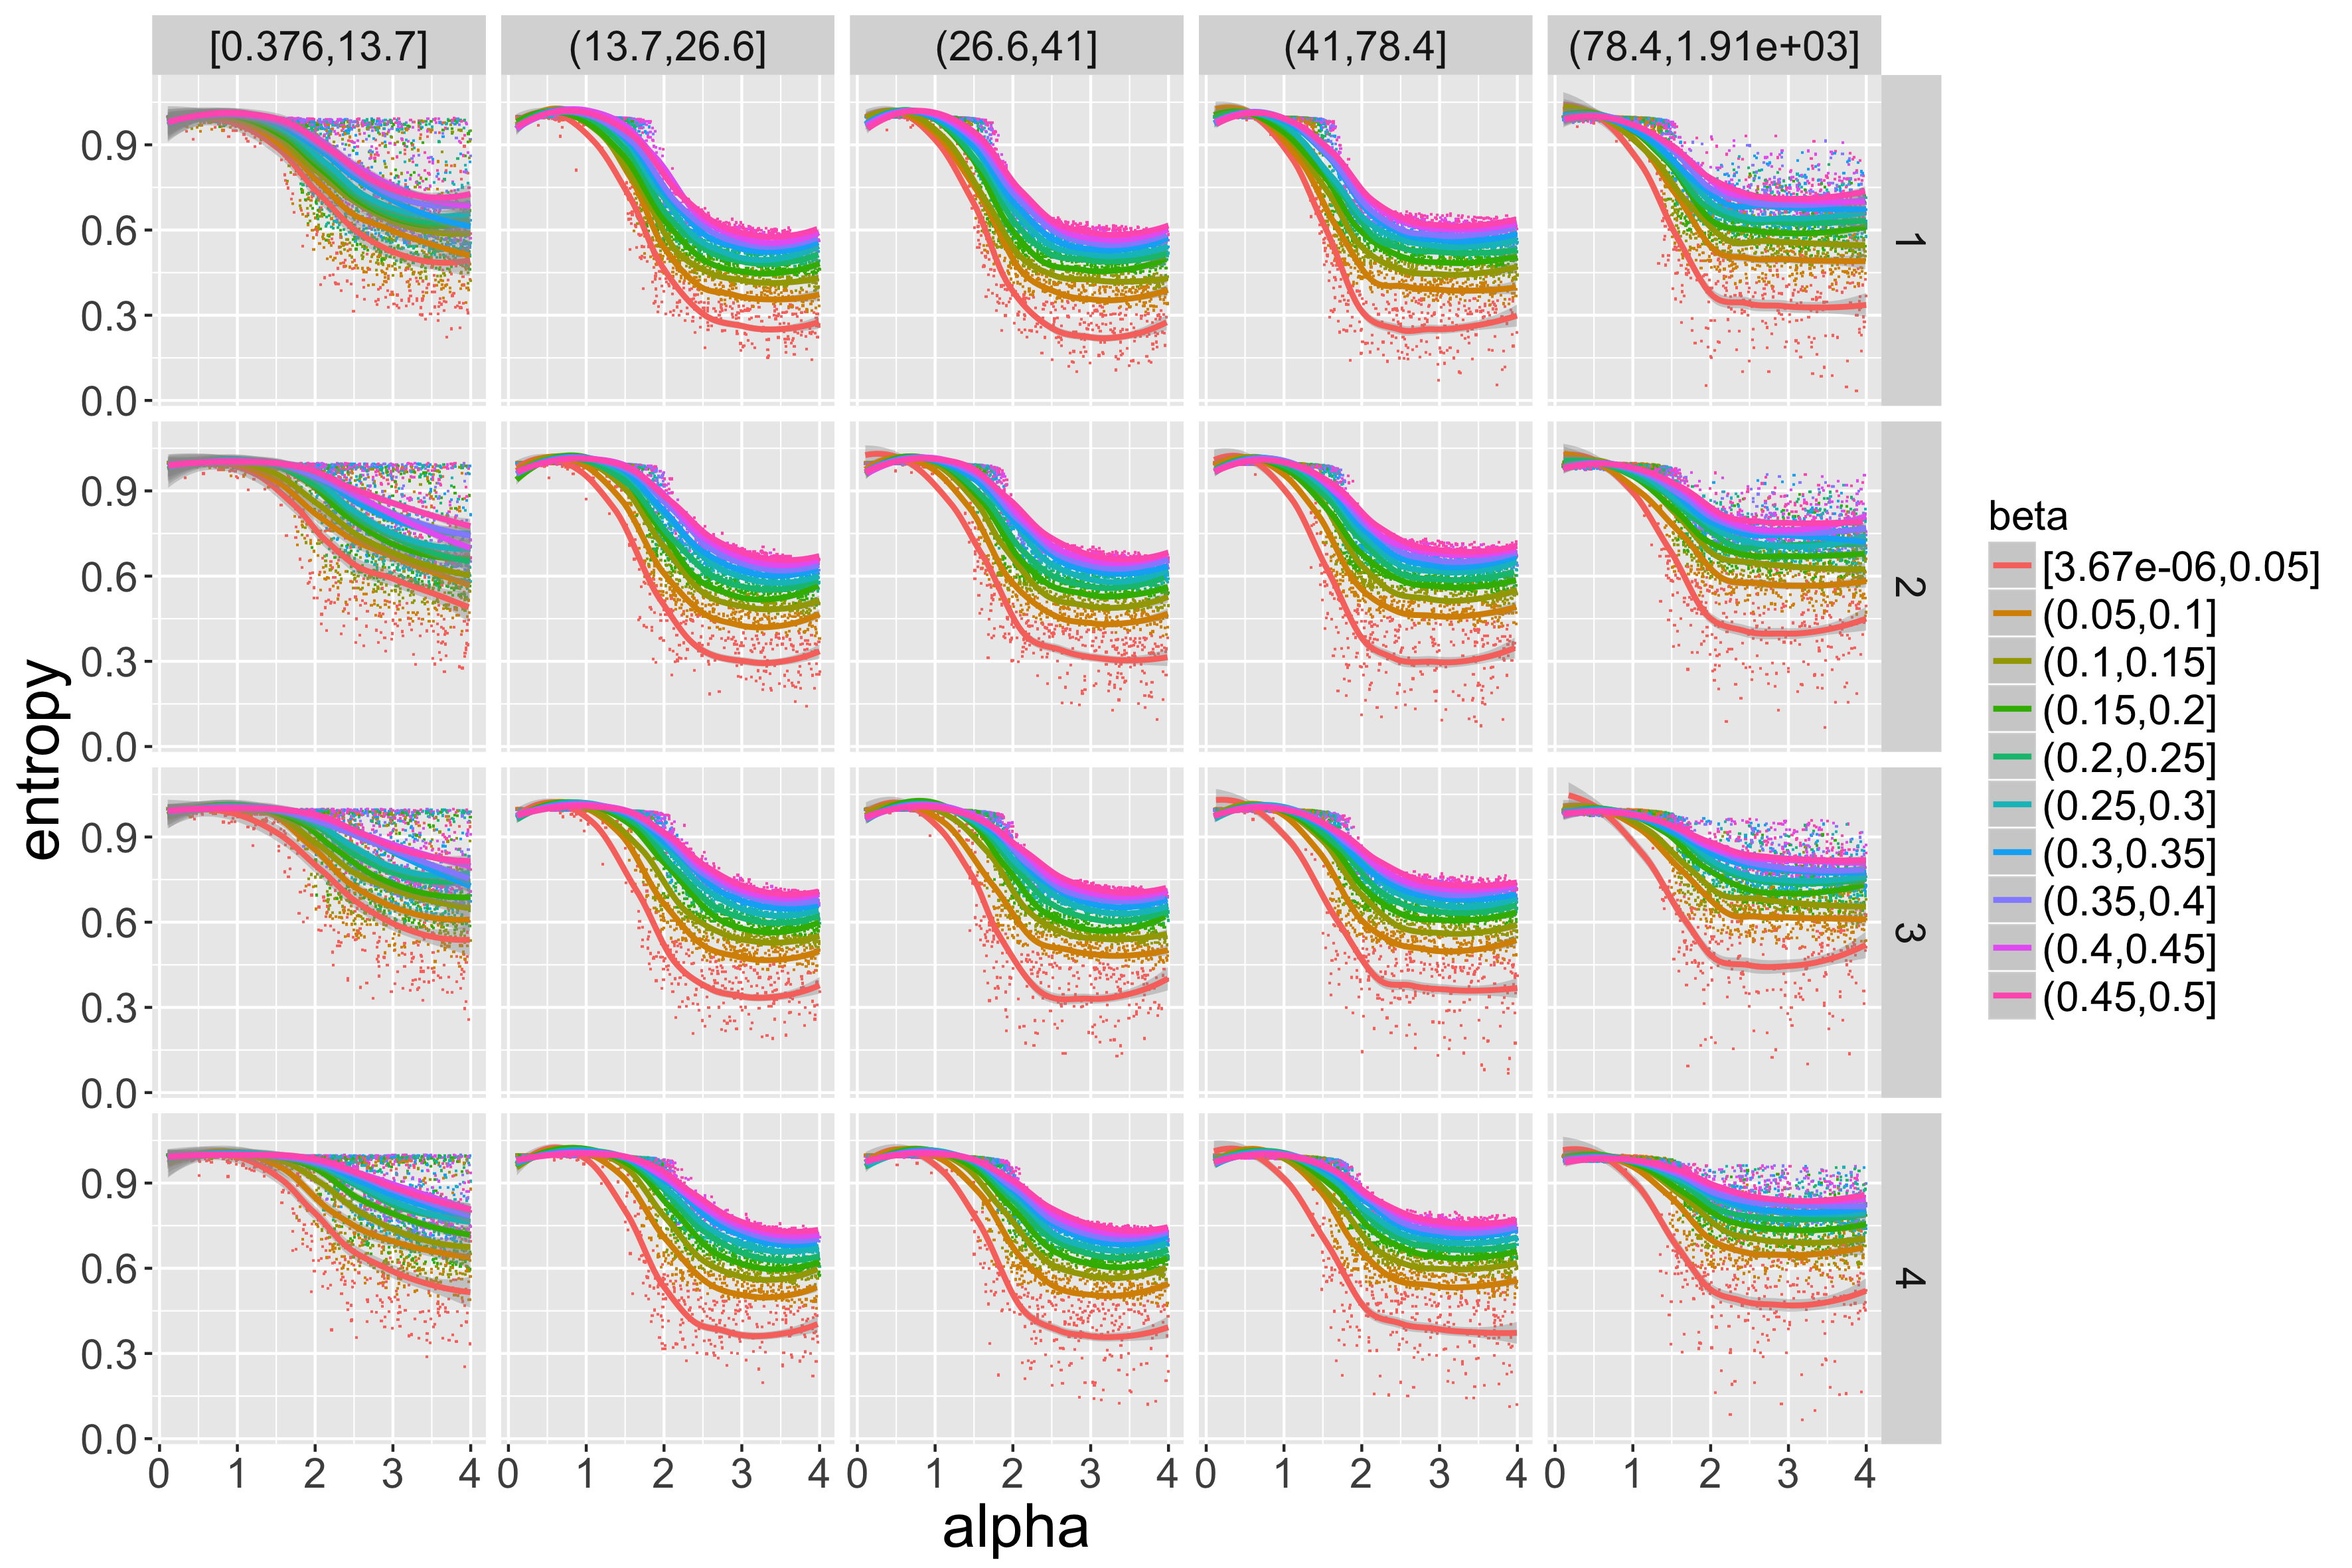
\includegraphics[width=\textwidth]{figuresraw/entropy_alpha}
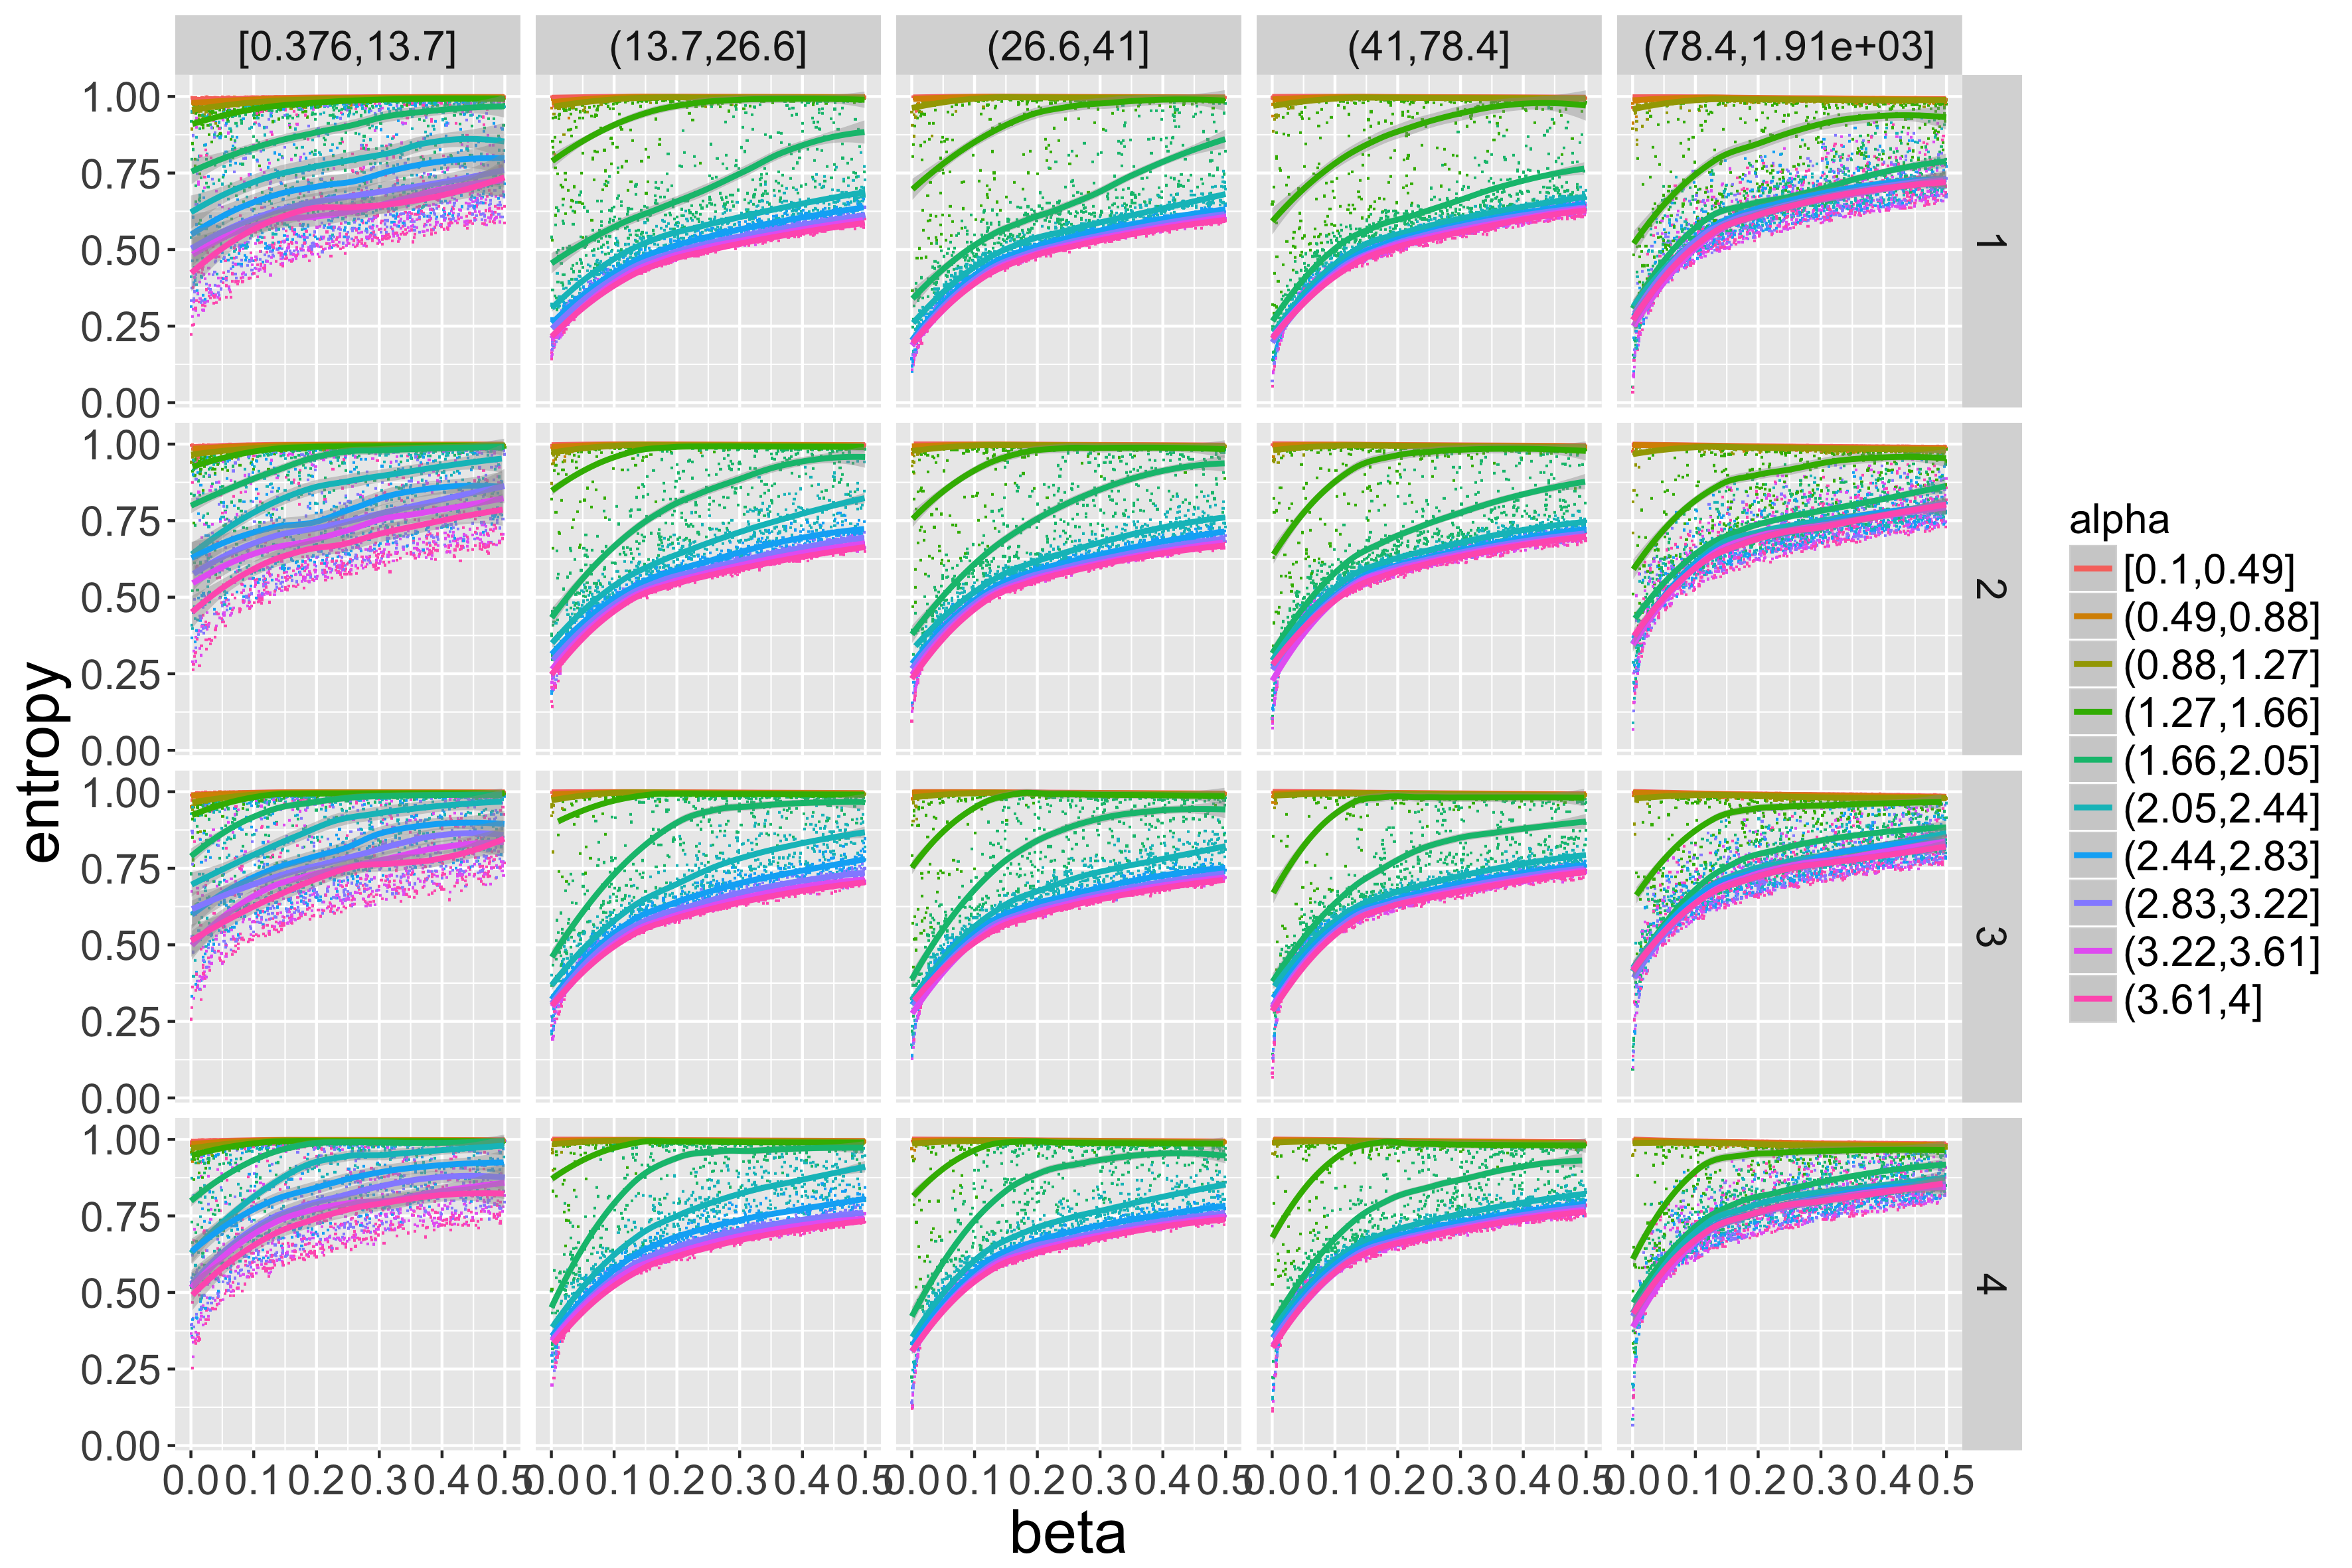
\includegraphics[width=\textwidth]{figuresraw/entropy_beta}
\caption{}
\label{}
\end{figure}
%%%%%%%%%%%%%%%%%%%%





\end{document}
